\section{AVL Trees}
If a binary tree is approximately \blue{balanced}, i.e.~if the left and right subtree of a binary tree $b$  have
roughly the same height, then the complexity of $b.\texttt{find}(k)$ will always be of the order
$\Oh\bigl(\ln(n)\bigr)$.  There are a number of different variations of
balanced binary trees.  Of these variations, the species of balanced binary trees that is the easiest to understand is
called an \href{https://en.wikipedia.org/wiki/AVL_tree}{AVL tree} \cite{adelson:62}.  AVL trees are 
named after their inventors \href{https://en.wikipedia.org/wiki/Georgy_Adelson-Velsky}{Georgy M.~Adelson-Velsky}
\index{Adelson-Velsky, Georgy Maximovich} 
(1922 -- 2014) and \href{https://en.wikipedia.org/wiki/Evgenii_Landis}{Evgenii~M.~Landis} (1921 -- 1997).
\index{Landis, Evgenii Mikhailovich}
In order to define these trees we need to define the \blue{height} of a binary tree formally:
\begin{enumerate}
\item $\texttt{Nil}.\texttt{height}() = 0$.
\item $\texttt{Node}(k,v,l,r).\texttt{height}() = 
       \max\bigl( l.\texttt{height}(), r.\texttt{height}() \bigr) + 1$. \eox
\end{enumerate}

\begin{Definition}[AVL-Tree] \hspace*{\fill} \\
{\em 
  The set $\AVL$ of \blue{AVL trees}\index{AVL tree} \index{$\mathcal{A}$, AVL tree} is defined inductively:
  \begin{enumerate}
  \item $\texttt{Nil} \in \AVL$.
  \item $\texttt{Node}(k,v,l,r) \in \AVL$ \quad iff 
        \begin{enumerate}
        \item $\texttt{Node}(k,v,l,r) \in \Bin$,
        \item $l, r \in \AVL$, \quad and
        \item $|l.\texttt{height}() - r.\texttt{height}()| \leq 1$.

              This condition is called the \blue{balancing condition}. \index{balancing condition}
        \end{enumerate}
        According to this definition, an AVL tree is an ordered binary tree such that for every node
        $\texttt{Node}(k,v,l,r)$ in this tree the height of the left subtree $l$ and the right
        subtree  $r$ differ at most by one.  \qed
  \end{enumerate}
}  
\end{Definition}

In order to specify the methods \emph{$\texttt{find}$}, \emph{$\texttt{insert}$}, and \emph{$\texttt{delete}$} for AVL trees we
adapt the recursive equations that we have used to define these functions for ordered binary trees.
In addition to those methods that we have already seen in the class $\texttt{Map}$ we will need the method
\\[0.2cm]
\hspace*{1.3cm} $\texttt{restore}: \Bin \rightarrow \AVL$. 
\\[0.2cm]
This method is used to restore the balancing condition at a given node if it has been violated by
either inserting or deleting an element.
The method call $b.\texttt{restore}()$ assumes that  $b$ is an ordered binary tree that satisfies
the balancing condition everywhere except possibly at its root. 
At the root, the height of the left subtree might differ from the height of the right subtree by at
most 2.  Hence, when the method $b.\texttt{restore}()$ is invoked we have either of the following
two cases:
\begin{enumerate}
\item $b = \texttt{Nil}$ \quad or
\item $b = \texttt{Node}(k,v,l,r) \wedge l \in \AVL \wedge r \in \AVL \wedge
       |l.\texttt{height}() - r.\texttt{height}()| \leq 2$.
\end{enumerate}
The method $\texttt{restore}$ is specified via conditional equations.
\begin{enumerate}
\item $\texttt{Nil}.\texttt{restore}() = \texttt{Nil}$,

      because the empty tree already is an  AVL tree.
\item $|l.\texttt{height}() - r.\texttt{height}()| \leq 1 \rightarrow 
       \texttt{Node}(k,v,l,r).\texttt{restore}() = \texttt{Node}(k,v,l,r)$.

      If the balancing condition is satisfied, then nothing needs to be done. 
\item $\begin{array}[t]{cl}
              & l_1.\texttt{height}() = r_1.\texttt{height}() + 2    \\ 
       \wedge & l_1 = \texttt{Node}(k_2,v_2,l_2,r_2)                 \\
       \wedge & l_2.\texttt{height}() \geq r_2.\texttt{height}()     \\[0.2cm]
       \rightarrow & \texttt{Node}(k_1,v_1,l_1,r_1).\texttt{restore}() = 
                     \texttt{Node}\bigl(k_2,v_2,l_2,\texttt{Node}(k_1,v_1,r_2,r_1)\bigr)
       \end{array}
      $

      The motivation for this equation can be found in Figure \ref{fig:casell}
      on page \pageref{fig:casell}.  The left part of this figure shows the state
      of the tree before it has been rebalanced.  Therefore, this part shows the tree
      \\[0.2cm]
      \hspace*{1.3cm}
      $\texttt{Node}(k_1,v_1, \texttt{Node}(k_2,v_2,l_2,r_2), r_1)$. 
      \\[0.2cm]
      The right part of Figure \ref{fig:casell} shows the effect of rebalancing.  
      This rebalancing results in the tree
      \\[0.2cm]
      \hspace*{1.3cm}
      $\texttt{Node}\bigl(k_2,v_2,l_2,\texttt{Node}(k_1,v_1,r_2,r_1)\bigr)$.
      \\[0.2cm]
      In Figure \ref{fig:casell} the label below the horizontal line of each node shows the height
      of the tree corresponding to this node.  For subtrees, the height is given below the name of
      the subtree.  For example,  $h$ is the height of the subtree 
      $l_2$, while $h-1$ is the height of the subtree $r_1$. The height of the subtree $r_2$
      is $h'$ and we know that $h' \leq h$.  As $\texttt{Node}(k_2,v_2,l_2,r_2)$ is an AVL tree and we know that
      $l_2.\texttt{height}() \geq r_2.\texttt{height}()$, we
      either have $h' = h$ or $h' = h-1$.

      The state shown in Figure \ref{fig:casell} can arise if either an element has been inserted
      in the left subtree $l_1$ or if an element has been deleted from the right subtree  $r_1$.

      \begin{figure}[!ht]
        \centering
        \framebox{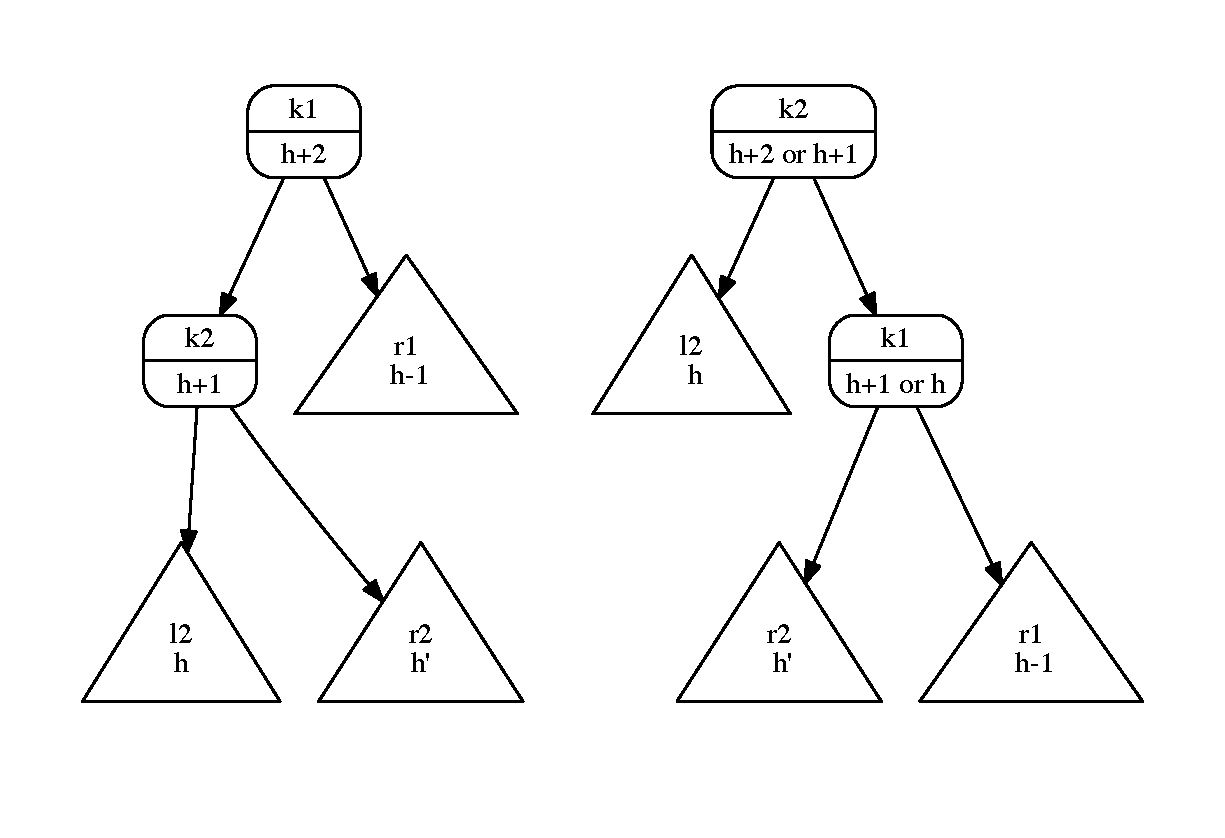
\epsfig{file=Abbildungen/casell.pdf,scale=0.7}} 
        \caption{An unbalanced tree and the corresponding rebalanced tree.}
        \label{fig:casell}
      \end{figure}
      We have to make sure that the tree shown in the right part of Figure
      \ref{fig:casell} is indeed an  AVL tree. With respect to the balancing condition this is
      easily verified.  The fact that the node containing the key $k_1$ has either the height
      $h$ or $h+1$ is a consequence of the fact that the height of $r_1$ is  $h-1$ while the height of $r_2$ is
      $h'$ and we know that $h' \in \{h, h-1\}$.

      In order to verify that the tree is ordered we can use the following inequation: 
      \\[0.2cm]
      \hspace*{1.3cm}
      $l_2 < k_2 < r_2 < k_1 < r_1$. 
      \hspace*{\fill} $(\star)$
      \\[0.2cm]
      Here we have used the following notation: If  $k$ is a key and  $b$ is a binary tree, then we write \\[0.2cm]
      \hspace*{1.3cm} $k < b$ \\[0.2cm]
      in order to express that  $k$ is smaller than all keys that occur in the tree  $b$.
      Similarly,  $b < k$ denotes the fact that all keys occurring in $b$ are less than the key
      $k$.  The inequation  $(\star)$ describes both the ordering of keys in the left part of Figure
      \ref{fig:casell} and in the right part of this figure.  Hence, the tree shown in the right
      part of Figure \ref{fig:casell} is ordered provided the tree in the left part is ordered to begin with.
\item $\begin{array}[t]{cl}
               & l_1.\texttt{height}() = r_1.\texttt{height}() + 2    \\ 
        \wedge & l_1 = \texttt{Node}(k_2,v_2,l_2,r_2)               \\
        \wedge & l_2.\texttt{height}() < r_2.\texttt{height}()     \\
        \wedge & r_2 = \texttt{Node}(k_3,v_3,l_3,r_3)               \\
        \rightarrow & \texttt{Node}(k_1,v_1,l_1,r_1).\texttt{restore}() = 
                      \texttt{Node}\bigl(k_3,v_3,\texttt{Node}(k_2,v_2,l_2,l_3),\texttt{Node}(k_1,v_1,r_3,r_1) \bigr)
        \end{array}
       $

       The left hand side of this equation is shown in Figure  \ref{fig:caselr} on page
       \pageref{fig:caselr}.  This tree can be written as
       \\[0.2cm]
       \hspace*{1.3cm} 
       $\texttt{Node}\bigl(k_1,v_1,\texttt{Node}(k_2,v_2,l_2,\texttt{Node}\bigl(k_3,v_3,l_3,r_3)\bigr),r_1\bigr)$. 
       \\[0.2cm]
       The subtrees $l_3$ and $r_3$ have either the height  $h$ or $h-1$.  Furthermore, at least one
       of these subtrees must have the height  $h$ for otherwise the subtree
       $\texttt{Node}(k_3,v_3,l_3,r_3)$ would not have the height $h+1$.
       
\begin{figure}[!ht]
  \centering
  \framebox{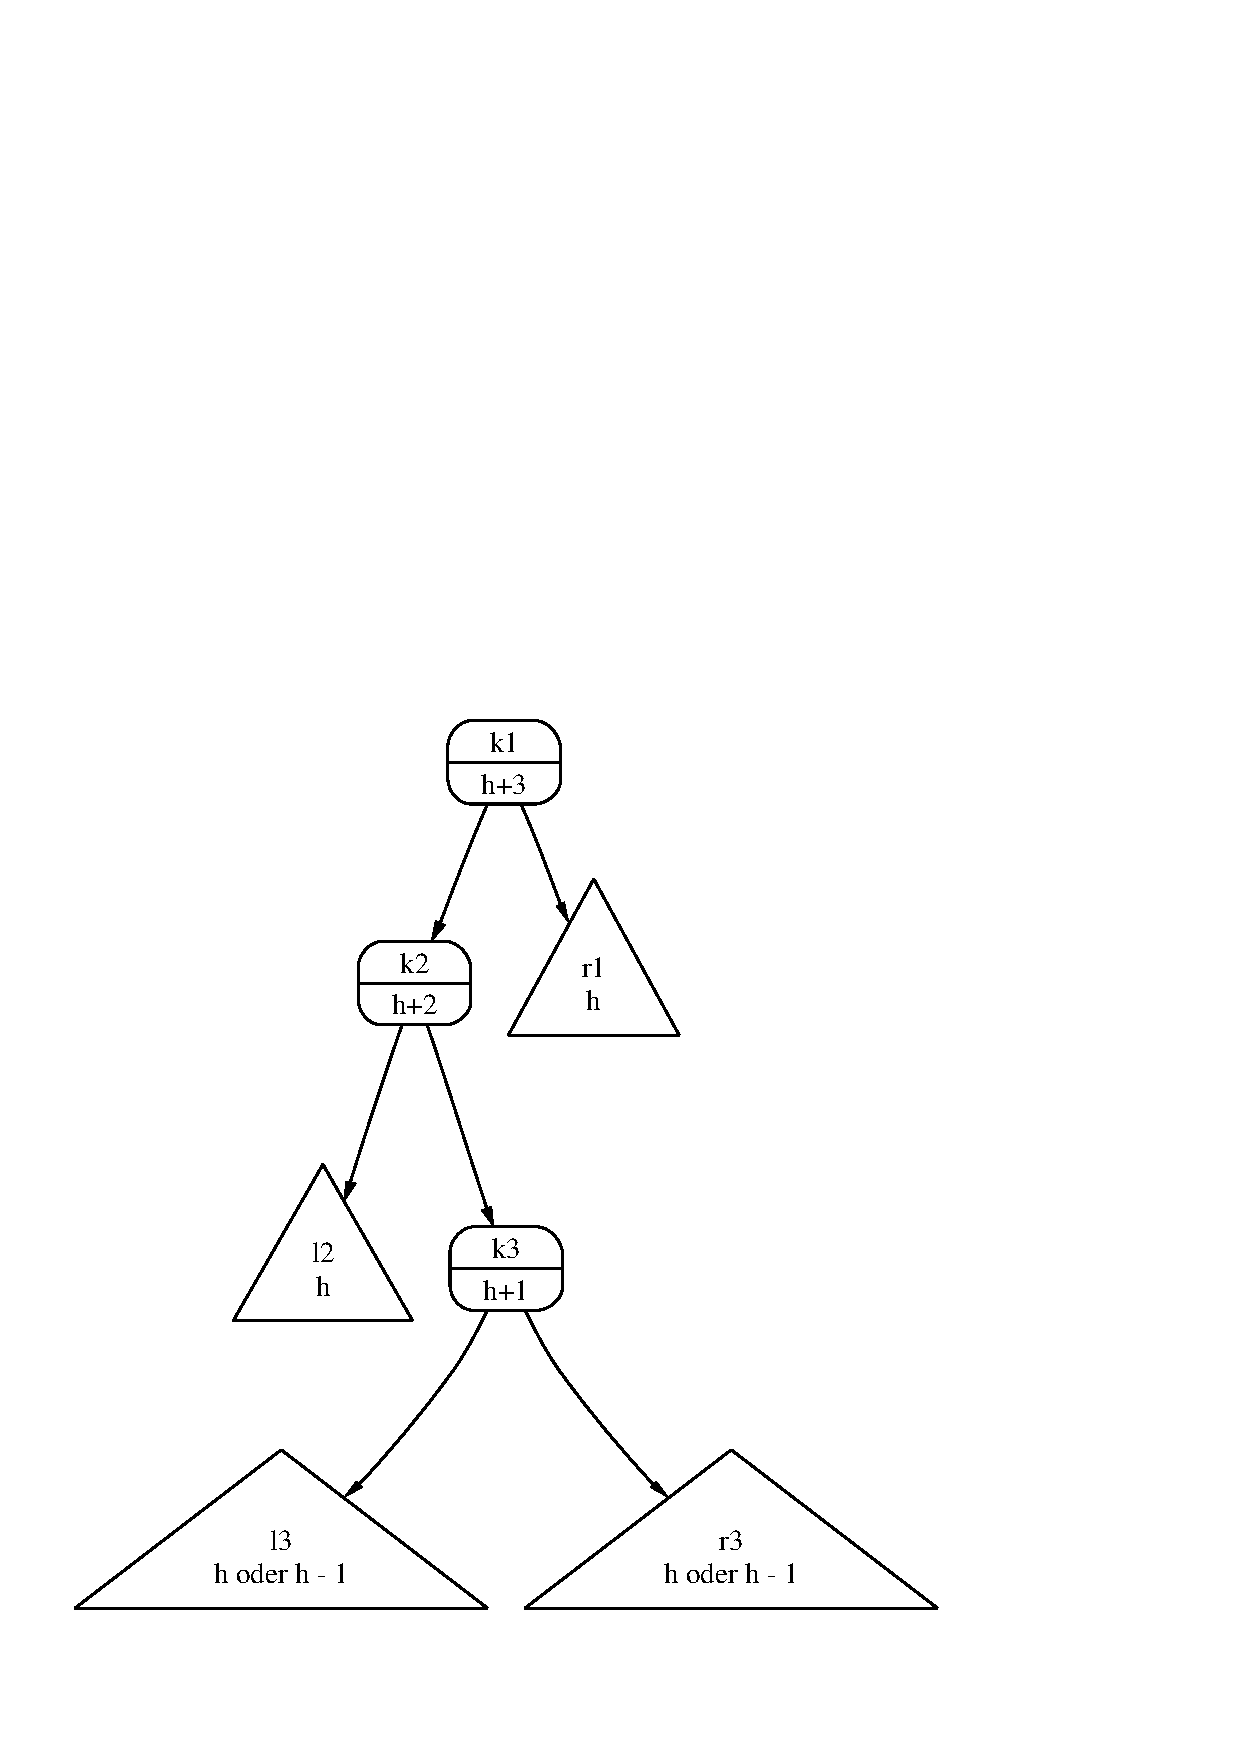
\epsfig{file=Abbildungen/caselr,scale=0.7}} 
  \caption{An unbalanced tree, second case.}
  \label{fig:caselr}
\end{figure}

     Figure \ref{fig:caselr-nach} on page \pageref{fig:caselr-nach} shows how the tree looks after
     rebalancing.  The tree shown in this figure has the form
     \\[0.2cm]
     \hspace*{1.3cm} 
     $\texttt{Node}\bigl(k_3,v_3,\texttt{Node}(k_2,v_2,l_2,l_3),\texttt{Node}(k_1,v_1,r_3,r_1) \bigr)$.


\begin{figure}[!ht]
  \centering
  \framebox{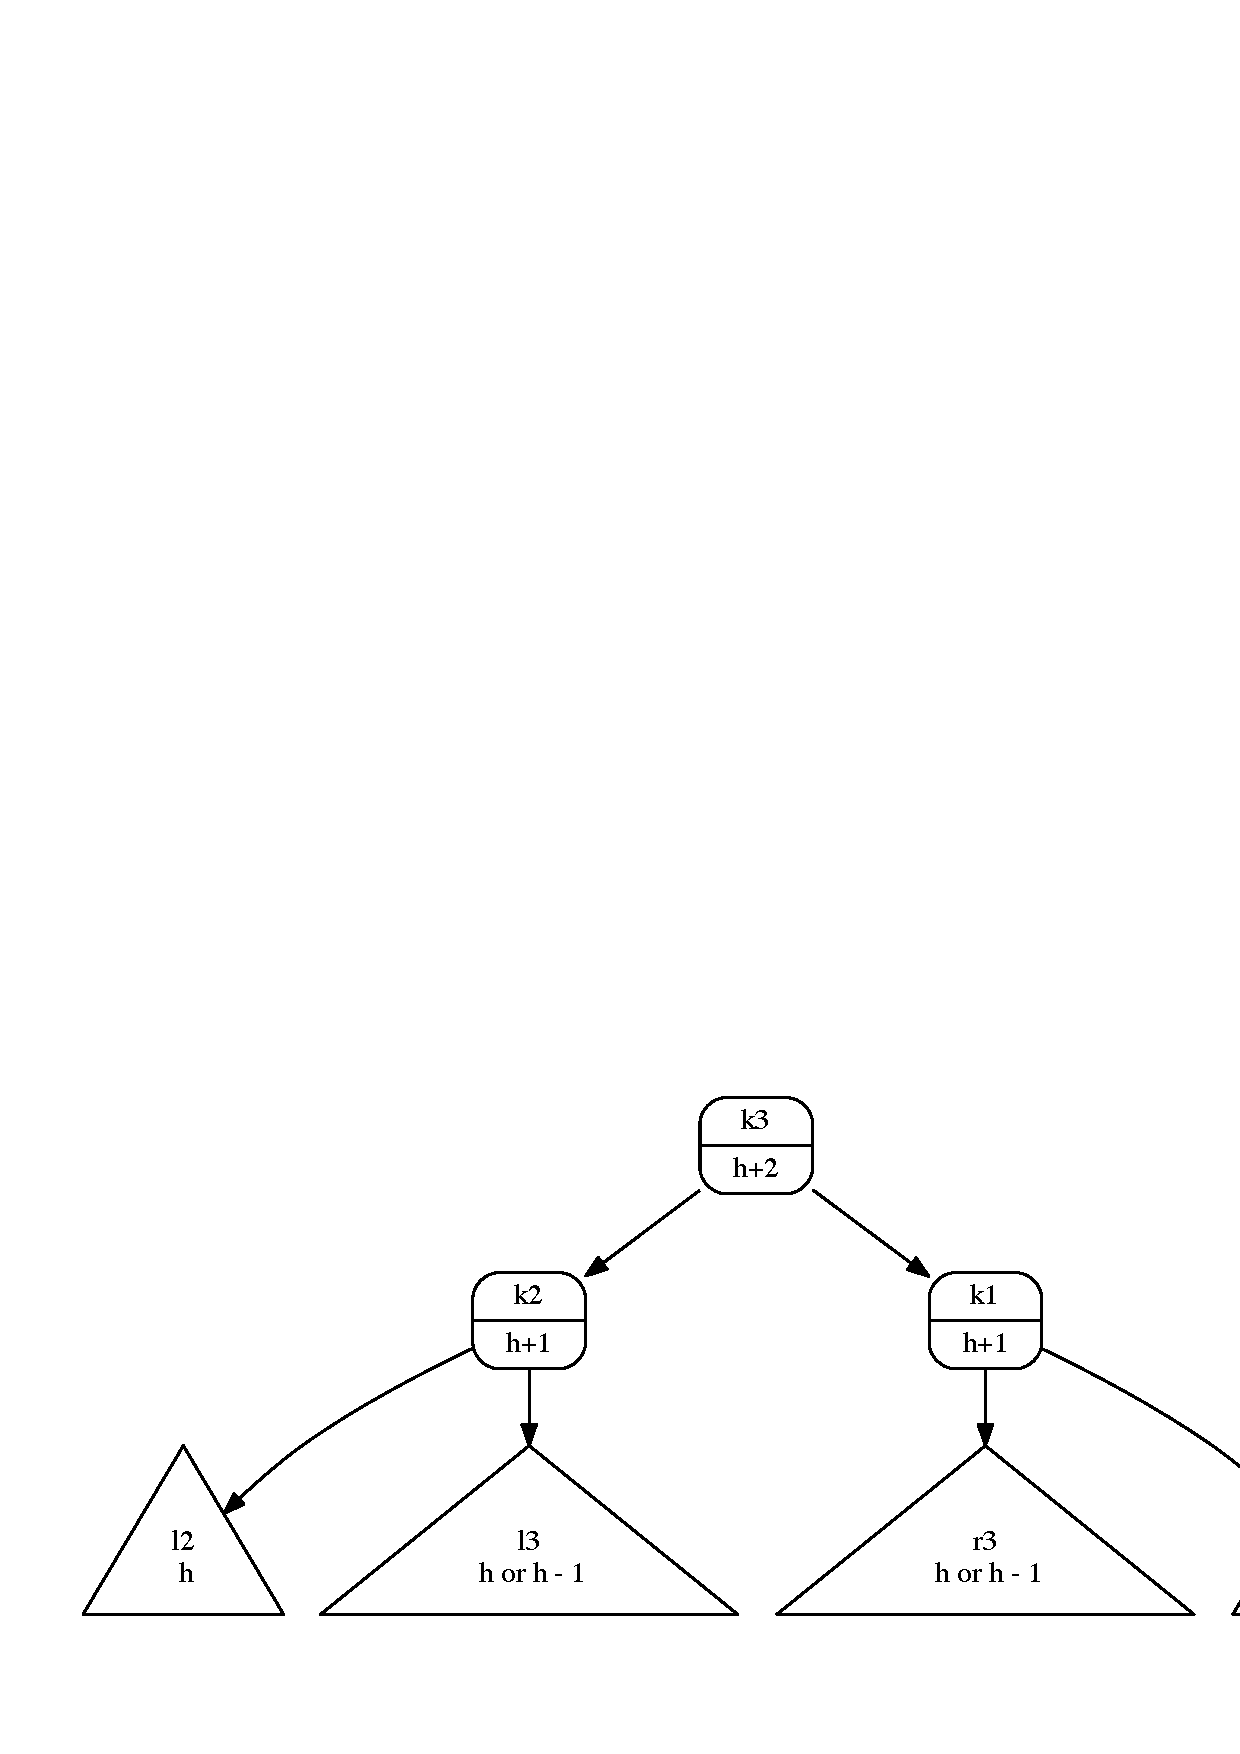
\epsfig{file=Abbildungen/caselr-nach,scale=0.7}} 
  \caption{The rebalanced tree in the second case.}
  \label{fig:caselr-nach}
\end{figure}

      The inequation describing the ordering of the keys both in the left subtree and in the right
      subtree is given as
      \\[0.2cm]
      \hspace*{1.3cm} $l_2 < k_2 < l_3 < k_3 < r_3 < k_1 < r_1$.

      There are two more cases where the height of the right subtree is bigger by more than 
      the height of the left subtree plus one.  These two cases are completely analogous to the two
      cases discussed previously.  Therefore we just state the corresponding equations without
      further discussion.
\item $\begin{array}[t]{cl}
              & r_1.\texttt{height}() = l_1.\texttt{height}() + 2    \\ 
       \wedge & r_1 = \texttt{Node}(k_2,v_2,l_2,r_2)               \\
       \wedge & r_2.\texttt{height}() \geq l_2.\texttt{height}()     \\[0.2cm]
       \rightarrow & \texttt{Node}(k_1,v_1,l_1,r_1).\texttt{restore}() = 
                     \texttt{Node}\bigl(k_2,v_2,\texttt{Node}(k_1,v_1,l_1,l_2),r_2\bigr)
       \end{array}
      $
\item $\begin{array}[t]{cl}
               & r_1.\texttt{height}() = l_1.\texttt{height}() + 2    \\ 
        \wedge & r_1 = \texttt{Node}(k_2,v_2,l_2,r_2)               \\
        \wedge & r_2.\texttt{height}() < l_2.\texttt{height}()     \\
        \wedge & l_2 = \texttt{Node}(k_3,v_3,l_3,r_3)               \\
        \rightarrow & \texttt{Node}(k_1,v_1,l_1,r_1).\texttt{restore}() = 
                      \texttt{Node}\bigl(k_3,v_3,\texttt{Node}(k_1,v_1,l_1,l_3),\texttt{Node}(k_2,v_2,r_3,r_2) \bigr)
        \end{array}
       $

\end{enumerate}
Now we are ready to specify the method  $\texttt{insert}()$ via recursive equations.
If we compare these equations to the equations we had given for unbalanced ordered binary trees we
notice that we only have to call the method $\texttt{restore}$ if the balancing condition might have
been violated.
\begin{enumerate}
\item $\texttt{Nil}.\texttt{insert}(k,v) = \texttt{Node}(k,v, \texttt{Nil}, \texttt{Nil})$.  
\item $\texttt{Node}(k, v_2, l, r).\texttt{insert}(k,v_1) = \texttt{Node}(k, v_1, l, r)$.
\item $k_1 < k_2 \rightarrow 
          \texttt{Node}(k_2, v_2, l, r).\texttt{insert}(k_1, v_1) =
          \texttt{Node}\bigl(k_2, v_2, l.\texttt{insert}(k_1,v_1), r\bigr).\texttt{restore}()$.
\item $k_1 > k_2 \rightarrow 
         \texttt{Node}(k_2, v_2, l, r).\texttt{insert}\bigl(k_1, v_1\bigr) = 
         \texttt{Node}\bigl(k_2, v_2, l, r.\texttt{insert}(k_1,v_1)\bigr).\texttt{restore}()$.
\end{enumerate}
The equations for  $\texttt{delMin}()$ change as follows:
\begin{enumerate}
\item $\texttt{Node}(k, v, \texttt{Nil}, r).\texttt{delMin}() = \langle r, k, v \rangle$.
\item $l\not= \texttt{Nil} \wedge \langle l',k_{min}, v_{min}\rangle := l.\texttt{delMin}() 
       \;\rightarrow$ \\[0.2cm]
       \hspace*{1.3cm} 
       $\texttt{Node}(k, v, l, r).\texttt{delMin}() = 
        \langle \texttt{Node}(k, v, l', r).\texttt{restore}(), k_{min}, v_{min} \rangle$.
\end{enumerate}
Finally, the equations for $\texttt{delete}$ are as follows:
\begin{enumerate}
\item $\texttt{Nil}.\texttt{delete}(k) = \texttt{Nil}$.
\item $\texttt{Node}(k,v,\texttt{Nil},r).\texttt{delete}(k) = r$.
\item $\texttt{Node}(k,v,l,\texttt{Nil}).\texttt{delete}(k) = l$.
\item $l \not= \texttt{Nil} \,\wedge\, r \not= \texttt{Nil} \,\wedge\, 
       \langle r',k_{min}, v_{min} \rangle := r.\texttt{delMin}()  \;\rightarrow$ \\[0.2cm]
      \hspace*{1.3cm}
      $\texttt{Node}(k,v,l,r).\texttt{delete}(k) = \texttt{Node}(k_{min},v_{min},l,r').\texttt{restore}()$.
\item $k_1 < k_2 \rightarrow \texttt{Node}(k_2,v_2,l,r).\texttt{delete}(k_1) = 
       \texttt{Node}\bigl(k_2,v_2,l.\texttt{delete}(k_1),r\bigr).\texttt{restore}()$.
\item $k_1 > k_2 \rightarrow \texttt{Node}(k_2,v_2,l,r).\texttt{delete}(k_1) = 
         \texttt{Node}\bigl(k_2,v_2,l,r.\texttt{delete}(k_1)\bigr).\texttt{restore}()$.
\end{enumerate}


\subsection{Implementing AVL-Trees in \textsl{Python}}
If we want to implement AVL-trees in \textsl{Python} then we have to decide how to compute the height
of the trees.  The idea is to store the height of every subtree in the corresponding node since it
would be inefficient if we would recompute this height every time we need it.  Therefore, we add a
member variable \texttt{mHeight} to our class map.
Figure \ref{fig:avl-tree.ipython:init} shows the constructor of the class \texttt{AVLTree}.  The variable
\texttt{mHeight} is defined in line 7.  It is initialised as $0$ since the constructor \texttt{\_\_init\_\_}
constructs an empty node.  

\begin{figure}[!ht]
  \centering
\begin{minted}[ frame         = lines, 
                framesep      = 0.3cm, 
                bgcolor       = sepia,
                numbers       = left,
                numbersep     = -0.2cm,
                xleftmargin   = 0.8cm,
                xrightmargin  = 0.8cm
              ]{python3}
    class AVLTree:
        def __init__(self):
            self.mKey    = None
            self.mValue  = None
            self.mLeft   = None
            self.mRight  = None
            self.mHeight = 0 
\end{minted}
\vspace*{-0.3cm}
  \caption{Outline of the class \texttt{map}.}
  \label{fig:avl-tree.ipython:init}
\end{figure}


Figure \ref{fig:avl-tree.ipython:find} shows the implementation of the function $\texttt{find}$.
Actually, the implementation is the same as the implementation in Figure
\ref{fig:binary-tree.py-1}.  The reason is that every AVL tree is also an ordered binary tree and
since searching for a key does not change the underlying tree there is no need to restore anything.

\begin{figure}[!ht]
\centering
\begin{minted}[ frame         = lines, 
                  framesep      = 0.3cm, 
                  firstnumber   = 1,
                  bgcolor = sepia,
                  numbers       = left,
                  numbersep     = -0.2cm,
                  xleftmargin   = 0.8cm,
                  xrightmargin  = 0.8cm,
                ]{python3}
    def find(self, key):
        if self.isEmpty():
            return
        elif self.mKey == key:
            return self.mValue
        elif key < self.mKey:
            return self.mLeft.find(key)
        else:
            return self.mRight.find(key)
\end{minted}
\vspace*{-0.3cm}
\caption{Implementation of the method $\texttt{find}$.}
\label{fig:avl-tree.ipython:find}
\end{figure}


Figure \ref{fig:avl-tree.ipython:insert} shows the implementation of the method $\texttt{insert}$.
If we compare this implementation with the implementation for ordered binary trees, we find three
differences.
\begin{enumerate}
\item When inserting into an empty tree, we now have to update the member variable \texttt{mHeight}
      to $1$.  This is done in line 7.
\item After inserting a key-value pair into the left subtree \texttt{mLeft}, it might be necessary to 
      rebalance the tree.  This is done in line 12.
\item Similarly, if we insert a key-value pair into the right subtree \texttt{mRight}, we have to rebalance 
      the tree.  This is done in line 15.
\end{enumerate}

\begin{figure}[!ht]
\centering
\begin{minted}[ frame         = lines, 
                  framesep      = 0.3cm, 
                  firstnumber   = 1,
                  bgcolor = sepia,
                  numbers       = left,
                  numbersep     = -0.2cm,
                  xleftmargin   = 0.8cm,
                  xrightmargin  = 0.8cm,
                ]{python3}
    def insert(self, key, value):
        if self.isEmpty():
            self.mKey    = key
            self.mValue  = value
            self.mLeft   = AVLTree()
            self.mRight  = AVLTree()
            self.mHeight = 1
        elif self.mKey == key:
            self.mValue = value
        elif key < self.mKey:
            self.mLeft.insert(key, value)
            self._restore()
        else:
            self.mRight.insert(key, value)
            self._restore()
\end{minted}
\vspace*{-0.3cm}
\caption{Implementation of the method $\texttt{insert}$.}
\label{fig:avl-tree.ipython:insert}
\end{figure}

Figure \ref{fig:avl-tree.ipython:delMin} shows the implementation of the method \texttt{delMin}.
The only change compared to the previous implementation for ordered binary trees is in line 7, where
we have to take care of the fact that the balancing condition might be violated after deleting the
smallest element in the left subtree.

\begin{figure}[!ht]
\centering
\begin{minted}[ frame         = lines, 
                framesep      = 0.3cm, 
                firstnumber   = 1,
                bgcolor = sepia,
                numbers       = left,
                numbersep     = -0.2cm,
                xleftmargin   = 0.8cm,
                xrightmargin  = 0.8cm,
              ]{python3}
    def _delMin(self):
        if self.mLeft.isEmpty():
            return self.mRight, self.mKey, self.mValue
        else:
            ls, km, vm = self.mLeft._delMin()
            self.mLeft = ls
            self._restore()
            return self, km, vm
\end{minted}
\vspace*{-0.3cm}
\caption{Implementation of \texttt{delMin}.}
\label{fig:avl-tree.ipython:delMin}
\end{figure}


Figure \ref{fig:avl-tree.ipython:delete} shows the implementation of the method $\texttt{delete}$ and the
implementation of the auxiliary method \texttt{update}.  Compared with Figure
\ref{fig:binary-tree.py-2} there are only three differences:
\begin{enumerate}
\item If we delete the key at the root of the tree, we replace this key with the smallest key in the
      right subtree. Since this key is deleted in the right subtree, the height of the right
      subtree might shrink and hence the balancing condition at the root might be violated.
      Therefore, we have to restore the balancing condition.  This is done in line 12.
\item If we delete a key in the left subtree, the height of the left subtree might shrink.
      Hence we have to rebalance the tree at the root in line 15.
\item Similarly, if we delete a key in the right subtree, we have to restore the balancing
      condition.  This is done in line 18.
\end{enumerate}
Since the method \texttt{update} replaces the current tree with either its left or right subtree and this
subtree is assumed to satisfy the balancing condition, there is no need for a call to \texttt{restore} in this
method. 

\begin{figure}[!ht]
\centering
\begin{minted}[ frame         = lines, 
                framesep      = 0.3cm, 
                firstnumber   = 1,
                bgcolor = sepia,
                numbers       = left,
                numbersep     = -0.2cm,
                xleftmargin   = 0.8cm,
                xrightmargin  = 0.8cm,
              ]{python3}
    def delete(self, key):
        if self.isEmpty():
            return
        if key == self.mKey:
            if self.mLeft.isEmpty():
                self._update(self.mRight)
            elif self.mRight.isEmpty():
                self._update(self.mLeft)
            else:
                self.mRight, self.mKey, self.mValue = \
                     self.mRight._delMin()
                self._restore()
        elif key < self.mKey:
            self.mLeft.delete(key)
            self._restore()
        else:
            self.mRight.delete(key)
            self._restore() 

    def _update(self, t):
        self.mKey    = t.mKey
        self.mValue  = t.mValue
        self.mLeft   = t.mLeft
        self.mRight  = t.mRight
        self.mHeight = t.mHeight            
\end{minted}
\vspace*{-0.3cm}
\caption{The methods $\texttt{delete}$ and \texttt{update}.}
\label{fig:avl-tree.ipython:delete}
\end{figure}
\begin{figure}[!ht]
\centering
\begin{minted}[ frame         = lines, 
                framesep      = 0.3cm, 
                firstnumber   = 1,
                bgcolor = sepia,
                numbers       = left,
                numbersep     = -0.2cm,
                xleftmargin   = 0.0cm,
                xrightmargin  = 0.0cm,
              ]{python3}
    def _restore(self):
        if abs(self.mLeft.mHeight - self.mRight.mHeight) <= 1:
            self._restoreHeight()
            return
        if self.mLeft.mHeight > self.mRight.mHeight:
            k1,v1,l1,r1 = self.mKey,self.mValue,self.mLeft,self.mRight
            k2,v2,l2,r2 = l1.mKey, l1.mValue, l1.mLeft, l1.mRight
            if l2.mHeight >= r2.mHeight:
                self._setValues(k2, v2, l2, createNode(k1,v1,r2,r1))
            else: 
                k3,v3,l3,r3 = r2.mKey,r2.mValue,r2.mLeft,r2.mRight
                self._setValues(k3, v3, createNode(k2, v2, l2, l3),
                                        createNode(k1, v1, r3, r1))
        elif self.mRight.mHeight > self.mLeft.mHeight:
            k1,v1,l1,r1 = self.mKey,self.mValue,self.mLeft,self.mRight
            k2,v2,l2,r2 = r1.mKey, r1.mValue, r1.mLeft, r1.mRight
            if r2.mHeight >= l2.mHeight:
                self._setValues(k2, v2, createNode(k1,v1,l1,l2), r2)
            else:
                k3,v3,l3,r3 = l2.mKey,l2.mValue,l2.mLeft,l2.mRight
                self._setValues(k3, v3, createNode(k1, v1, l1, l3),
                                        createNode(k2, v2, r3, r2))
        self._restoreHeight()
    
    def _setValues(self, k, v, l, r):
        self.mKey   = k
        self.mValue = v
        self.mLeft  = l
        self.mRight = r
    
    def _restoreHeight(self):
        self.mHeight = max(self.mLeft.mHeight, self.mRight.mHeight)+1
\end{minted}
\vspace*{-0.3cm}
\caption{The implementation of \texttt{restore} and \texttt{restoreHeight}.}
\label{fig:avl-tree.ipython:restore}
\end{figure}


Figure \ref{fig:avl-tree.ipython:restore} shows the implementation of the function \texttt{restore}.
It is this method that makes most of the difference between ordered binary trees and AVL trees.  Let
us discuss this method line by line.
\begin{enumerate}
\item In line 2 we check whether the balancing condition is satisfied.  If we are lucky,  this test 
      is successful and hence we do not need to restore the structure of the tree.  However, we
      still need to maintain the height of the tree since it is possible that variable
      \texttt{mHeight} no longer contains the correct height.  For example, assume that the left subtree
      initially has a height that is bigger by one than the height of the right subtree.  Assume
      further that we have deleted a node in the left subtree so that its height shrinks.  Then the
      balancing condition is still satisfied, as now the left subtree and the right subtree have the
      same height.  However, the height of the complete tree has also shrunk by one and therefore, 
      the variable \texttt{mHeight} needs to be decremented.  This is done via the auxiliary method
      \texttt{restoreHeight}.  This method is defined in line 31 and it recomputes \texttt{mHeight}
      according to the definition of the height of a binary tree.
\item If the check in line 2 fails, then we know that the balancing condition is violated.
      However, we do not yet know which of the two subtrees is bigger.  

      If the test in line 5 succeeds, then the left subtree must have a height that is bigger by
      two than the height of the right subtree.  In order to be able to use the same variable names 
      as the variable names given in the equations discussed in the previous subsection, we define
      the variables \texttt{k1}, \texttt{v1}, \texttt{l1}, \texttt{r1}, \texttt{k2}, \texttt{v2}, \texttt{l2},
      and \texttt{r2} in line 6 and 7 so that these variable names correspond exactly to the variable names
      used in the Figures \ref{fig:casell} and \ref{fig:caselr}.
\item Next, the test in line 8 checks whether we have the case that is depicted in Figure
      \ref{fig:casell}.  In this case, Figure \ref{fig:casell} tells us that the key \texttt{k2}
      has to move to the root.  The left subtree is now \texttt{l2}, while the right subtree is a
      new node that has the key \texttt{k1} at its root.  This new node is created by the call
      of the function \texttt{createNode} in line 9.  The function \texttt{createNode} is shown in
      Figure \ref{fig:avl-tree.ipython:createNode} on page \pageref{fig:avl-tree.ipython:createNode}.
\item If the test in line 8 fails, the right subtree is bigger than the left subtree and we are in 
      the case that is depicted in Figure \ref{fig:caselr}.  We have to create the tree that is
      shown in Figure \ref{fig:caselr-nach}.  To this end we first define the variables 
      \texttt{k3}, \texttt{v3}, \texttt{l3}, and \texttt{r3} in a way that these variables
      correspond to the variables shown in Figure \ref{fig:caselr}.  Next, we create the tree
      that is shown in Figure \ref{fig:caselr-nach}.
\item Line 14 deals with the case that the right subtree is bigger than the left subtree. 
      As this case is analogous to the case covered in line 5 to line 13, we won't discuss this case
      any further.
\item Finally, we recompute the variable \texttt{mHeight} since it is possible that the old value is
      no longer correct.
\end{enumerate}


\begin{figure}[!ht]
\centering
\begin{minted}[ frame         = lines, 
                framesep      = 0.3cm, 
                firstnumber   = 1,
                bgcolor = sepia,
                numbers       = left,
                numbersep     = -0.2cm,
                xleftmargin   = 0.8cm,
                xrightmargin  = 0.8cm,
              ]{python3}
    def createNode(key, value, left, right):
        node         = AVLTree()
        node.mKey    = key
        node.mValue  = value
        node.mLeft   = left
        node.mRight  = right
        node.mHeight = max(left.mHeight, right.mHeight) + 1
        return node
\end{minted}
\vspace*{-0.3cm}
\caption{Implementation of \texttt{createNode}.}
\label{fig:avl-tree.ipython:createNode}
\end{figure}

The function \texttt{createNode} shown in Figure \ref{fig:avl-tree.ipython:createNode}
constructs a node with given left and right subtrees.  In fact, this method serves as a second
constructor for the class \texttt{map}.  The implementation should be obvious.


\subsection{Analysis of the Complexity of AVL Trees}
Next, we analyse the complexity of AVL trees in the worst case.  In order to do this we have to know
what the worst case actually looks like.  Back when we only had ordered binary trees the worst case was the case where
the tree had degenerated into a list.  Now, the worst case is the case where the tree is as slim as
it can possibly be while still satisfying the definition of an AVL tree.  Hence the worst case
happens if the tree has a given height $h$ but the number of keys stored in the tree is as small as
possible.  To investigate trees of this kind, let us define  $b_h(k)$ as an AVL tree that has the following three
properties:
\begin{enumerate}[(a)]
\item The height of $b_h(k)$ is $h$.
\item The number of keys stored in $b_h(k)$ is minimal among all other AVL trees of height $h$.  
\item All keys stored in  $b_h(k)$ are natural number that are bigger than  $k$.

      In order for the expression $b_h(k)$ to be clearly defined we demand that keys
      in $b_h(k)$ are as small as possible.
\end{enumerate}
For our investigation of the complexity, both the keys and the values do not really matter.  The only problem
is that we have to ensure that the tree $b_h(k)$ is an ordered tree.
Before we can present the definition of $b_h(k)$ we need to define the auxiliary function
 $\texttt{maxKey}()$.  This function has the signature 
\\[0.2cm]
\hspace*{1.3cm}
$\texttt{maxKey}:\mathcal{B} \rightarrow \texttt{Key} \cup \{ \Omega \}$.
\\[0.2cm]
Given a non-empty ordered binary tree  $b$, the expression $b.\texttt{maxKey}()$ returns the biggest
key stored in $b$.  The expression  $b.\texttt{maxKey}()$ is defined by induction on $b$:
\begin{enumerate}
\item $\texttt{Nil}.\texttt{maxKey}() = \Omega$,
\item $\texttt{Node}(k,v,l,\texttt{Nil}).\texttt{maxKey}() = k$,
\item $r \not= \texttt{Nil} \rightarrow \texttt{Node}(k,v,l,r).\texttt{maxKey}() = r.\texttt{maxKey}()$.
\end{enumerate}
Now we are ready to define the trees  $b_h(k)$ by induction on  $h$.
\begin{enumerate}
\item $b_0(k) = \texttt{Nil}$,

      because there is only one AVL tree of height $0$ and this is the tree $\texttt{Nil}$.
\item $b_1(k) = \texttt{Node}(k+1,0,\texttt{Nil}, \texttt{Nil})$,

      since, if we abstract from the actual keys and values, there is exactly one AVL tree of height
      $1$.
\item $b_{h+1}(k).\texttt{maxKey}() = l \rightarrow 
       b_{h+2}(k) = \texttt{Node}\bigl(l+1,\,0,\,b_{h+1}(k),\,b_h(l+1)\bigr)$.

      In order to construct an AVL tree of height $h+2$ that contains the minimal number of keys 
      possible we first construct the AVL tree $b_{h+1}(k)$ which has height  $h+1$ and which stores as few
      key as possible given its height.  Next, we determine the biggest key $l$ in this tree. 
      Now to construct $b_{h+2}(k)$ we take a node with the key $l+1$ as the root.
      The left subtree of this node is $b_{h+1}(k)$, while the right subtree is $b_h(l+1)$.
      Since $l$ is the biggest key in $b_{h+1}(k)$, all key in the left subtree of
      $b_{h+2}(k)$ are indeed smaller than the key $l+1$ at the root.  Since all keys in
      $b_h(l+1)$ are bigger than $l+1$, the keys in the right subtree are bigger than the key at the
      root.  Therefore, $b_{h+2}(k)$ is an ordered binary tree.

      Furthermore, $b_{h+2}(k)$ is an AVL tree of height $h+2$ since the height of the left subtree
      is $h+1$ and the height of the right subtree is $h$.  Also, this tree is as slim as
      any AVL tree can possibly get, since if the left subtree has height $h+1$ the right subtree
      must at least have height $h$ in order for the whole tree to be an AVL tree.
\end{enumerate}
Let us denote the number of keys stored in a binary tree $b$ as  $\#\,b$.  Furthermore, we define
\\[0.2cm]
\hspace*{1.3cm}
$c_h := \#\, b_h(k)$
\\[0.2cm]
to be the number of keys in the tree $b_h(k)$.  We will soon see that 
$\#\,b_h(k)$ does not depend on the number $k$ and therefore $c_h$ does not depend on $k$.  Starting
from the definition of $b_h(k)$ we find the following equations for $c_h$:
\begin{enumerate}
\item $c_0 = \#\, b_0(k) = \#\, \texttt{Nil} = 0$,
\item $c_1 = \#\, b_1(k) = \#\, \texttt{Node}(k+1,0,\texttt{Nil}, \texttt{Nil}) = 1$, 
\item$\begin{array}[t]{lcl}
       c_{h+2} & = & \#\, b_{h+2}(k) \\
               & = & \#\,\texttt{Node}\bigl(l+1,\,0,\,b_{h+1}(k),\,b_h(l+1)\bigr) \\
               & = & \#\, b_{h+1}(k) + \#\, b_h(l+1) + 1 \\
               & = & c_{h+1} + c_h + 1.
       \end{array}$
\end{enumerate}
Hence we have found the \href{https://en.wikipedia.org/wiki/Recurrence_relation}{recurrence equation}
\\[0.2cm]
\hspace*{1.3cm}
$c_{h+2} = c_{h+1} + c_h + 1 \quad \mbox{with initial values $c_0 = 0$ and $c_1 = 1$}.$
\\[0.2cm]
This also validates our claim that $c_h$ does not depend on $k$.  Due to the presence of the number $1$ on the
right hand side of this recurrence equation, this recurrence equation is an 
\blue{inhomogeneous recurrence equation}.  In order to solve this recurrence
equation we first solve the corresponding \blue{homogeneous recurrence equation} 
\\[0.2cm]
\hspace*{1.3cm}
$a_{h+2} = a_{h+1} + a_h$
\\[0.2cm]
using the \href{https://en.wikipedia.org/wiki/Ansatz}{ansatz}
\\[0.2cm]
\hspace*{1.3cm}
$a_h = \lambda^h$.
\\[0.2cm]
Substituting $a_h = \lambda^h$ into the recurrence equation for $a_h$ leaves us with the equation
\\[0.2cm]
\hspace*{1.3cm}
$\lambda^{h+2} = \lambda^{h+1} + \lambda^{h}$.
\\[0.2cm]
Dividing by $\lambda^h$ leaves the quadratic equation
\\[0.2cm]
\hspace*{1.3cm}
$\lambda^2 = \lambda + 1$
\\[0.2cm]
which can be rearranged as
\\[0.2cm]
\hspace*{1.3cm}
$\lambda^2 - 2 \cdot \lambda \cdot \frac{1}{2} = 1$.
\\[0.2cm]
Adding $\frac{1}{4}$ on both sides of this equation completes the square on the left hand side:
\\[0.2cm]
\hspace*{1.3cm}
$\bigl(\lambda - \frac{1}{2}\bigr)^2 = \frac{5}{4}$. 
\\[0.2cm]
From this we conclude 
\\[0.2cm]
\hspace*{1.3cm}
$\lambda = \frac{1}{2} \cdot \bigl(1 + \sqrt{5}\bigr) \;\vee\; \lambda = \frac{1}{2} \cdot \bigl(1 - \sqrt{5}\bigr)$.
\\[0.2cm]
Let us therefore define 
\\[0.2cm]
\hspace*{1.3cm}
$\lambda_1 =  \frac{1}{2} \cdot (1 + \sqrt{5}) \approx  1.618034$ \quad and \quad 
$\lambda_2 = \frac{1}{2} \cdot (1 - \sqrt{5}) \approx -0.618034$.
\\[0.2cm]
In order to solve the \blue{inhomogeneous recurrence equation} for $c_h$ we try the ansatz
\\[0.2cm]
\hspace*{1.3cm}
$c_h = d$ \quad for some constant $d$.
\\[0.2cm]
Substituting this ansatz into the recurrence equation for $c_h$ yields
\\[0.2cm]
\hspace*{1.3cm}
$d = d + d + 1$
\\[0.2cm]
from which we conclude that $d = -1$.  The solution for $c_h$ is now a linear combination of the solutions for
the corresponding homogeneous recurrence equation to which we have to add the solution for the inhomogeneous equation:
\\[0.2cm]
\hspace*{1.3cm}
$c_h = \alpha \cdot \lambda_1^h + \beta \cdot \lambda_2^h + d =\alpha \cdot \lambda_1^h + \beta \cdot \lambda_2^h - 1$.
\\[0.2cm]
Here, the values of $\alpha$ and $\beta$ can be found by setting $h=0$ and $h=1$ and using the
initial conditions $c_0 = 0$ and $c_1 = 1$.  This results in
the following system of linear equations for  $\alpha$ and $\beta$:
\\[0.2cm]
\hspace*{1.3cm}
$0 = \alpha + \beta - 1$ \quad and \quad
$1 = \alpha \cdot \lambda_1 + \beta \cdot \lambda_2 - 1$.
\\[0.2cm]
From the first equation we find $\beta = 1-\alpha$ and substituting this result into the second equation
gives
\\[0.2cm]
\hspace*{1.3cm}
$2 = \alpha \cdot \lambda_1 + (1-\alpha) \cdot \lambda_2$.
\\[0.2cm]
Solving this equation for $\alpha$ gives
\\[0.2cm]
\hspace*{1.3cm}
$2 - \lambda_2 = \alpha \cdot (\lambda_1 - \lambda_2)$
\\[0.2cm]
Now it just so happens that $\lambda_1 - \lambda_2 = \sqrt{5}$ and, furthermore, $2 - \lambda_2 = \lambda_1^2$.
We prove only the second claim, since the first is easy to verify.  We have the following
chain of equivalences:
$$
\begin{array}{crcl}
                  & 2 - \lambda_2 & = & \lambda_1^2            \\[0.2cm]
  \Leftrightarrow & 2 - \lambda_2 & = & \lambda_1 + 1          \\[0.2cm]
  \Leftrightarrow & 1             & = & \lambda_1 + \lambda_2  \\[0.2cm]
  \Leftrightarrow & 1             & = &\frac{1}{2} \cdot (1 + \sqrt{5}) + \frac{1}{2} \cdot (1 - \sqrt{5}) 
\end{array}
$$
Since the last equation is obviously true, the first is also true.
Hence, we have found
\\[0.2cm]
\hspace*{1.3cm}
$\ds \alpha = \frac{2 - \lambda_2}{\lambda_1 - \lambda_2} = \frac{1}{\sqrt{5}} \cdot \lambda_1^2$.
\\[0.2cm]
From this, a straightforward calculation using the fact that $\beta = 1 - \alpha$ shows that 
\\[0.2cm]
\hspace*{1.3cm}
$\ds \beta  = -\frac{1}{\sqrt{5}} \cdot \lambda_2^2$.
\\[0.2cm]
Therefore, $c_h$ is given by the following equation:
\\[0.2cm]
\hspace*{1.3cm}
$c_h = \ds \frac{1}{\sqrt{5}} \cdot \left( \lambda_1^{h+2} - \lambda_2^{h+2} \right) -1$.  
\\[0.2cm]
As we have  $|\lambda_2| < 1$, the value of  $\ds\lambda_2^{h+2}$ isn't important for big
values of $h$.  Therefore, for big values of $h$, the minimal number  $n$ of keys in a tree of
height  $h$ is approximately given by the formula \\[0.2cm]
\hspace*{1.3cm} $n \approx \ds \frac{1}{\sqrt{5}} \lambda_1^{h+2} - 1$. \\[0.2cm]
In order to solve this equation for  $h$ we take the logarithm of both side.  Then we have
\\[0.2cm]
\hspace*{1.3cm}
$\log_2(n+1) = (h+2) \cdot \log_2(\lambda_1) - \frac{1}{2}\cdot \log_2(5)$.
\\[0.2cm]
Adding  $\frac{1}{2}\cdot \log_2(5)$ gives
\\[0.2cm]
\hspace*{1.3cm}
$\log_2(n+1) + \frac{1}{2}\cdot \log_2(5) = (h+2) \cdot \log_2(\lambda_1)$.
\\[0.2cm]
Let us divide this inequation by  $\log_2(\lambda_1)$.  Then we get
\\[0.4cm]
\hspace*{1.3cm}
$\ds \bruch{\log_2(n+1) + \frac{1}{2}\cdot \log_2(5)}{\log_2(\lambda_1)} = h+2$.
\\[0.2cm]
Solving this equation for  $h$ gives the result 
\\[0.4cm]
\hspace*{1.3cm} 
$
\begin{array}[t]{lcl}
h & = & \ds \frac{\log_2(n+1) + \frac{1}{2}\cdot \log_2(5)}{\log_2(\lambda_1)} - 2 \\[0.4cm]
  & = & \ds \frac{1}{\log_2(\lambda_1)}\cdot \log_2(n) + \Oh(1) \\[0.5cm]
  & \approx & 1,44 \cdot \log_2(n) + \Oh(1).
\end{array} 
$
\\[0.2cm]
However, the height $h$ is the maximal number of comparisons needed to find a given key.
Hence, for AVL trees the complexity of $b.\texttt{find}(k)$ is logarithmic even in the worst case.
Figure 
\ref{fig:avl-worst-case} presents an  AVL tree of height 6 where the number of keys is minimal.



\begin{figure}[!ht]
  \centering
  \framebox{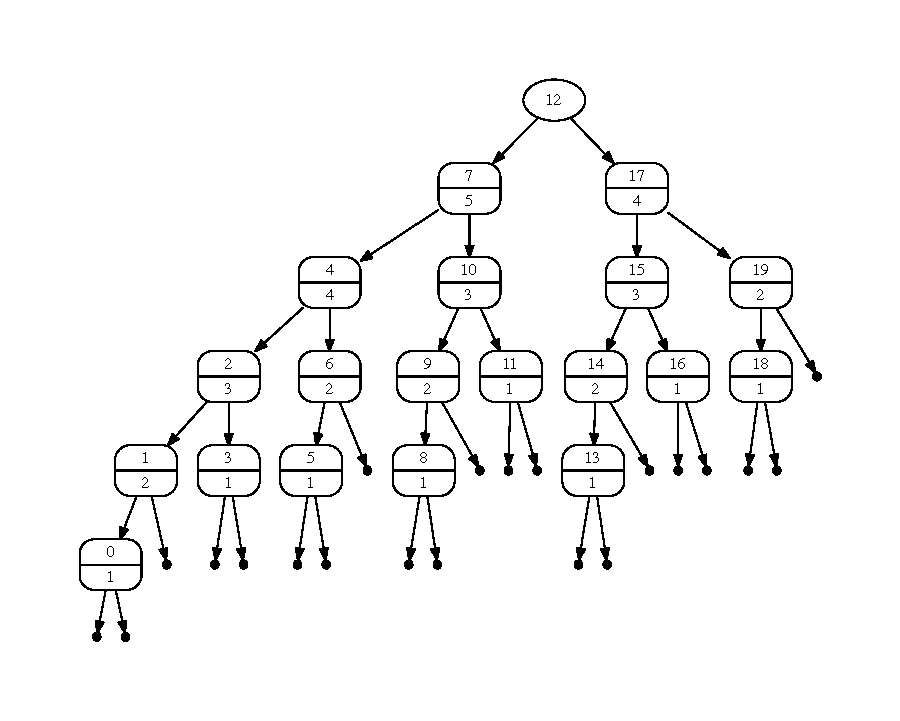
\epsfig{file=Abbildungen/avl}} 
  \caption{An AVL tree of height 6 that is as slim as possible.}
  \label{fig:avl-worst-case}
\end{figure}

\subsection{Improvements}
In practice, 
\href{https://en.wikipedia.org/wiki/Red-black_trees}{red-black trees} \index{red-black tree}
are slightly faster than \textsc{AVL} trees.  Similar to
\textsc{AVL} trees, a  red-black tree
  is an ordered binary tree that is approximately balanced.  Nodes are either black or red.
The children of a red node have to be black.  In order to keep red-black trees approximately
balanced, a \blue{relaxed height} of a tree is defined.  Red nodes do not contribute to the relaxed
height of a tree.  The left and right subtree of every node of a red-black tree are required to have the same 
relaxed height.  A detailed and very readable exposition of red-black trees is given by Sedgewick
\cite{sedgewick:2011}.  Red-black trees have been invented by Leonidas L.~Guibas and 
\href{https://en.wikipedia.org/wiki/Robert_Sedgewick_(computer_scientist)}{Robert Sedgewick} \cite{guibas:78}.

\exercise
Instead of using AVL trees, another alternative to implement a map is to use 
\href{https://en.wikipedia.org/wiki/2-3_tree}{2-3 trees}.  \index{2-3 tree}
Below we describe a simplified version of these trees.  These trees do not store any values.  Hence, instead
of implementing maps, these trees implement sets. They are built using the following constructors:
\begin{enumerate}
\item $\texttt{Nil}$ is a 2-3 tree that represents the empty set.
\item $\texttt{Two}(l, k, r)$ is a 2-3 tree provided
      \begin{enumerate}[(a)]
      \item $l$ is a 2-3 tree,
      \item $k$ is a key,
      \item $r$ is a 2-3 tree,
      \item all keys stored in $l$ are less than k and all keys stored in $r$ are bigger than $k$,
            i.e.~we have
            \\[0.2cm]
            \hspace*{1.3cm}
            $l < k < r$.
      \item $l$ and $r$ have the same height.
      \end{enumerate}
      A node of the form  $\texttt{Two}(l, k, r)$ is called a \blue{2-node}.  Except for the fact
      that there is no value, a 2-node is
      interpreted in the same way as we have interpreted the term $\texttt{Node}(k, v, l, r)$.
\item $\texttt{Three}(l, k_1, m, k_2, r)$ is a 2-3 tree provided
      \begin{enumerate}[(a)]
      \item $l$, $m$, and $r$ are 2-3 trees,
      \item $k_1$ and $k_2$ are keys,
      \item $l < k_1 < m < k_2 < r$,
      \item $l$, $m$, and $r$ have the same height.
      \end{enumerate}
      A node of the form  $\texttt{Three}(l, k_1, m, k_2, r)$ is called a \blue{3-node}.
\end{enumerate}
In order to keep 2-3 trees balanced when inserting new keys, we use a fourth constructor of the form
\\[0.2cm]
\hspace*{1.3cm}
$\texttt{Four}(l,k_1,m_l, k_2, m_r, k_3, r)$.
\\[0.2cm]
A term of the form $\texttt{Four}(l,k_1,m_l, k_2, m_r, k_3, r)$ is a \blue{2-3-4} tree iff
\begin{enumerate}
\item $l$, $m_l$, $m_r$, and $r$ are 2-3 trees,
\item $k_1$, $k_2$, and $k_3$ are keys,
\item $l < k_1 < m_l < k_2 < m_r < k_3 < r$,
\item $l$, $m_l$, $m_r$, and $r$ all have the same height.
\end{enumerate}
Nodes of this form are called 4-nodes and the key $k_2$ is called the \blue{middle key}.
Trees containing 4-nodes are called \blue{2-3-4} trees.
When a new key is inserted into a 2-3 tree, the challenge is to keep the tree balanced.  The easiest
case is the case where the tree has the form
\\[0.2cm]
\hspace*{1.3cm}
$\texttt{Two}(\texttt{Nil}, k, \texttt{Nil})$.
\\[0.2cm]
In this case, the 2-node is converted into a 3-node.  If the tree has the form 
\\[0.2cm]
\hspace*{1.3cm}
$\texttt{Three}(\texttt{Nil}, k_1, \texttt{Nil}, k_2, \texttt{Nil})$,
\\[0.2cm]
the 3-node is temporarily transformed into a 4-node.  Next, the middle key of this node is lifted up
to its parent node.  For example, suppose we insert the key 3 into the tree
\\[0.2cm]
\hspace*{1.3cm}
$\texttt{Two}(\texttt{Two}(\texttt{Nil}, 1, \texttt{Nil}), 2, \texttt{Three}(\texttt{Nil}, 4, \texttt{Nil}, 5, \texttt{Nil}))$.
\\[0.2cm]
In this case, the key 3 needs to be inserted to the left of the key 4.  This yields the temporary tree 
\\[0.2cm]
\hspace*{1.3cm}
$\texttt{Two}(\texttt{Two}(\texttt{Nil}, 1, \texttt{Nil}), 2, \texttt{Four}(\texttt{Nil}, 3, \texttt{Nil}, 4, \texttt{Nil}, 5, \texttt{Nil}))$,
\\[0.2cm]
where the right subtree is the 4-node $\texttt{Four}(\texttt{Nil}, 3, \texttt{Nil}, 4, \texttt{Nil}, 5, \texttt{Nil})$.
Since this is not a 2-3 tree, we need to lift the middle key 4 to its parent node.  This results in
the new tree
\\[0.2cm]
\hspace*{1.3cm}
$\texttt{Three}(\texttt{Two}(\texttt{Nil}, 1, \texttt{Nil}), 2, \texttt{Two}(\texttt{Nil}, 3, \texttt{Nil}), 4, \texttt{Two}(\texttt{Nil}, 5, \texttt{Nil}))$.
\\[0.2cm]
This tree is a 2-3 tree.  In this example we have been lucky since the parent of the 4-node was
a 2 node and therefore we could transform it into a 3-node.  If the parent node instead is a 3-node,
it has to be transformed into a temporary 4-node.  Then, the middle key of this 4-node has to be
lifted up recursively to its parent.  
\begin{enumerate}[(a)]
\item Specify a method $t.\texttt{member}(k)$ that checks whether the key $k$ occurs in the 2-3 tree
      $t$.  You should use recursive equations to specify  $t.\texttt{member}(k)$.
\item Specify a method $t.\texttt{insert}(k)$ that inserts the key $k$ into the 2-3 tree
      $t$.  You should use three auxiliary functions to implement \texttt{insert}:
      \begin{enumerate}
      \item $t.\texttt{ins}(k)$ takes a 2-3 tree $t$ and a key $k$ and inserts the key $k$ into $t$.
            It returns a 2-3-4 tree that has at most one 4-node.  Unless the tree $t$ has a height of $1$, this
            4-node has to be a child of the root node.  The function \texttt{ins} is recursive and uses the
            function \texttt{restore} that is described next.
            Furthermore, the height of the tree $t.\mathtt{ins}(k)$ has to be the same as the height of the tree $t$.
      \item $t.\texttt{restore}()$ takes a 2-3-4 tree $t$ that has at most one 4-node, which has to be a child
            of the root.  It returns a 2-3-4 tree that has at most one 4-node.  This 4-node has to be the root node.
            Furthermore, the height of the tree $t.\mathtt{restore}()$ has to be the same as the height of the tree $t$.
      \item $t.\texttt{grow}()$ takes a 2-3-4 tree $t$ that has at most one 4-node, which has to be the root
            node of the tree.  It returns an equivalent 2-3 tree.  The height of this tree is either the same
            as the height of $t$ or it is the height of $t$ plus $1$.
      \end{enumerate}
      Having defined these auxiliary functions, the function \texttt{insert} can then be computed as follows:
      \\[0.2cm]
      \hspace*{1.3cm}
      $t.\texttt{insert}(k) = t.\texttt{ins}(k).\texttt{restore}().\texttt{grow}()$.
\item Implement 2-3 trees in \textsl{Python}.
\item \textbf{Optional}: Specify a method $t.\texttt{delete}(k)$ that deletes the key $k$ in the tree $t$.

      In order to implement the function \texttt{delete}, it is necessary to define 1-2-3 trees.
      In addition to both 2-nodes and 3-nodes, these trees also have 1-nodes.  These nodes come into existence
      when a key is deleted from a 2-node:  Deleting the key $k$ from the node
      \\[0.2cm]
      \hspace*{1.3cm}
      $\texttt{Two}(\texttt{Nil}, k, \texttt{Nil})$
      \\[0.2cm]
      creates the 1-node $\texttt{One}(\texttt{Nil})$.
\end{enumerate}
Prof. Lyn Turbak has written a helpful
\href{http://www.cs.princeton.edu/~dpw/courses/cos326-12/ass/2-3-trees.pdf}{paper} describing 2-3 trees in more
depth.  This paper gives a graphical presentation of the \texttt{insert} and \texttt{delete} operations.

\paragraph{History:}
According to \cite{cormen:09}, 2-3 trees have been invented by
\href{https://en.wikipedia.org/wiki/John_Hopcroft}{John Hopcroft} in 1970.  John Hopcroft received the 1986
Turing Award. 



\section{Tries}
Often, the keys of a map are strings.  For example, when you search with 
\href{https://www.google.com}{\blue{G}\red{o}\orange{o}\blue{g}\green{l}\red{e}}, you are using
a string as a key to lookup information that is stored in a gigantic map provided by Google.
As another example, in an electronic phone book the keys are names and therefore strings.  
There is a species of search trees that is particularly well adapted to the case that the keys are
strings.  These search trees are known as \href{https://en.wikipedia.org/?title=Trie}{tries}.  
The name is derived from the word
\blue{re\underline{trie}val}.  In order to be able to distinguish between \blue{tries} and
\blue{trees} we have to pronounce  \blue{trie}  so that it rhymes with \blue{pie}.   The data
structure of tries has been proposed 1959 by Ren\'e de la Briandais \cite{briandais:59}.

Tries are also trees, but in contrast to a binary tree where every node has two children, in a trie a
node can have as many children as there are characters in the alphabet that is used to represent the
strings.  In order to define tries formally we assume that the following is given:
\begin{itemize}
\item $\Sigma$ is finite set of \blue{characters}. $\Sigma$ is called the
      \blue{alphabet}. 
\item $\Sigma^*$ is the set of all \blue{strings} that are built from the characters of $\Sigma$.
      Formally, a string is just a list of characters.  If we have $w \in \Sigma^*$, then we write $w = cr$
      if $c$ is the first character of $w$ and if $r$ the string that remains if we remove the first
      character from $w$.
\item $\varepsilon$ denotes the empty string.
\item $\texttt{Value}$ is the set of all the values that can be associated with the keys.  
\end{itemize}
The set $\mathbb{T}$ of all tries \index{trie} is defined inductively using the constructor \\[0.2cm]
\hspace*{1.3cm} 
$\texttt{Node}: \texttt{Value} \times \texttt{List}(\Sigma) \times
\texttt{List}(\mathbb{T}) \rightarrow \mathbb{T}$. 
\\[0.2cm]
The inductive definition of the set $\mathbb{T}$ \index{$\mathbb{T}$} has only a single clause: If
\begin{enumerate}[(a)]
\item $v \in \texttt{Value} \cup \{\Omega\}$,
\item $C\!s = [c_1, \cdots, c_n] \in \texttt{List}(\Sigma)$ is a list of different characters of length
      $n$ and,
\item $T\!s = [t_1, \cdots, t_n] \in \texttt{List}(\mathbb{T})$ is a list of  tries of the same length $n$, 
\end{enumerate}
then we have 
\\[0.2cm]
\hspace*{1.3cm}  $\texttt{Node}(v, C\!s, T\!s) \in \mathbb{T}$.  
\\[0.2cm]
As there is only one clause in this definition, you might ask how this inductive definition gets started.
The answer is that the base case of this inductive definition is the case where
$n=0$ since in that case the lists  $C\!s$ and $T\!s$ are both empty.

In order to specify the semantics of a trie of the form $\texttt{Node}(v,C,T)$ 
we specify a function
\\[0.2cm]
\hspace*{1.3cm} 
$\texttt{find}: \mathbb{T} \times \Sigma^* \rightarrow \texttt{Value} \cup \{ \Omega\}$
\\[0.2cm]
that takes a trie and a string as arguments.  For a trie $t$ and a string $s$, the expression $t.\texttt{find}(s)$ returns the
value that is associated with the key $s$ in $t$.  The expression
$\texttt{Node}(v,C\!s,T\!s).\texttt{find}(s)$ is defined by induction on the length of the  string $s$:
\begin{enumerate}
\item $\texttt{Node}(v, C\!s, T\!s).\texttt{find}(\varepsilon) = v$.

      The value associated with the empty string $\varepsilon$ is stored at the root of the trie.
\item $c = c_i \rightarrow 
       \texttt{Node}(v, [c_1, \cdots, c_n], [t_1, \cdots, t_n]).\texttt{find}(cr) = t_i.\texttt{find}(r)
      $

      The trie $\texttt{Node}(v, [c_1, \cdots, c_n], [t_1, \cdots, t_n])$ associates a value with
      the key $cr$ if the list $[c_1, \cdots, c_n]$ has a position $i$ such that $c$ equals $c_i$
      and, furthermore, the trie  $t_i$ associates a value with the key  $r$.
\item $ c \not\in C\!s \rightarrow
       \texttt{Node}(v, C\!s, T\!s).\texttt{find}(cr) = \Omega
      $

      If $c$ does not occur in the list $C\!s$, then the trie $\texttt{Node}(v, C\!s, T\!s)$ does not store a value for
      the key $cr$.
\end{enumerate}

\begin{figure}[!ht]
  \centering
  \framebox{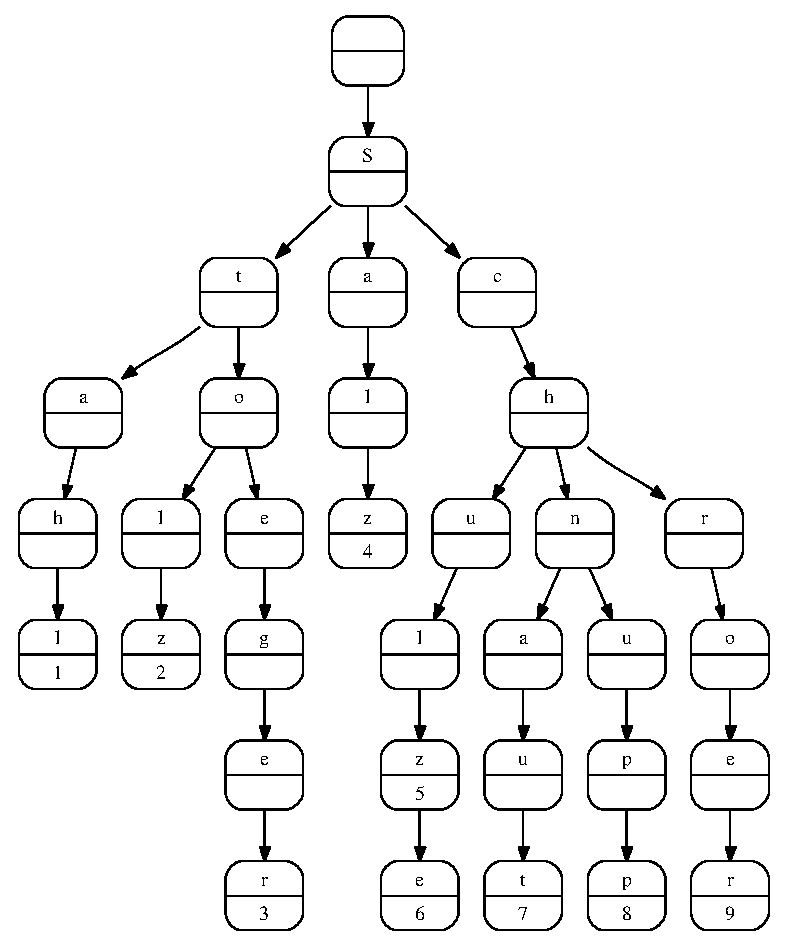
\epsfig{file=Abbildungen/trie}} 
  \caption{A trie storing some numbers.}
  \label{fig:trie}
\end{figure}

Graphically, tries are represented as trees.  Since it would be unwieldy to label the nodes of these
trees with the lists of characters corresponding to these nodes, we use a trick:  In order to
visualize a node of the form \\[0.2cm]
\hspace*{1.3cm} 
$\texttt{Node}(v, [c_1, \cdots, c_n], [t_1, \cdots, t_n])$ \\[0.2cm]
we draw a rectangle with rounded corners.  This rectangle is split into two parts by a horizontal line.
If the value  $v$ that is stored in this node is different from $\Omega$, then $v$ is
written in the lower part of the rectangle.  The label that we put in the upper half of the rectangle
depends on the parent of the node.  We will explain how this label is computed in a moment.
The node itself has $n$ different children.  These $n$ children are the tries
$t_1$, $\cdots$, $t_n$.  The node at the root of the trie $t_i$ is labelled with the character $c_i$,
i.e.~the rectangle that represents this node carries the label $c_i$ in its upper half.

In order to clarify these ideas, Figure  \ref{fig:trie} on page \pageref{fig:trie} shows a trie
mapping some strings to numbers.  The mapping depicted in this tree can be written as a \textsl{Python}
dictionary: 
\\[0.2cm]
\hspace*{1.3cm} $ \bigl\{ \texttt{'Stahl'}: 1, \texttt{'Stolz'}: 2, \texttt{'Stoeger'}: 3, \texttt{'Salz'}: 4, \texttt{'Schulz'}: 5$, \\[0.2cm]
\hspace*{1.5cm} $         \texttt{'Schulze'}: 6, \texttt{'Schnaut'}: 7, \texttt{'Schnupp'}: 8, \texttt{'Schroer'}: 9\bigr\}$. \\[0.2cm]
Since the node at the root has no parent, the upper half of  the rectangle representing the root is
always empty.  In the example shown in Figure \ref{fig:trie}, the lower half of this rectangle is also empty
because the trie doesn't associate a value with the empty string.  In this example, the root node corresponds
to the term  
\\[0.2cm]
\hspace*{1.3cm}
 $\texttt{Node}(\Omega,[\texttt{'S'}], [t])$. 
\\[0.2cm]
Here,  $t$ denotes the trie that is labelled with the character  \texttt{'S'} at its root.
This trie can then be represented by the term  \\[0.2cm]
\hspace*{1.3cm} 
$\texttt{Node}(\Omega,[\texttt{'t'},\texttt{'a'},\texttt{'c'}], [t_1, t_2, t_3])$. \\[0.2cm]
This trie has three children that are labelled with the characters  \texttt{'t'}, \texttt{'a'}, and \texttt{'c'}.

\subsection{Insertion in Tries}
Next, we present formulas that describe how new values can be inserted into existing tries,
i.e.~we specify the method $\texttt{insert}$.  The signature of $\texttt{insert}$ is given as follows:
\\[0.2cm]
\hspace*{1.3cm}
$\texttt{insert}: \mathbb{T} \times \Sigma^* \times \texttt{Value} \rightarrow \mathbb{T}$.
\\[0.2cm]
The result of evaluating \\[0.2cm]
\hspace*{1.3cm} 
$\texttt{Node}(v_1, [c_1, \cdots, c_n], [t_1, \cdots, t_n]).\texttt{insert}(w, v_2)$
\\[0.2cm]
for a string $w\in \Sigma^*$ and a value $v_2 \in \texttt{Value}$ is defined by induction on the
length of $w$.
\begin{enumerate}
\item $\texttt{Node}(v_1,L,T).\texttt{insert}(\varepsilon, v_2) = \texttt{Node}(v_2,L,T)$,
  
      If a new value $v_2$ is associated with the empty string $\varepsilon$, then the old value
      $v_1$, which had been stored at the root before, is overwritten.
\item $\texttt{Node}\bigl(v_1,[c_1,\cdots,c_i,\cdots,c_n], [t_1,\cdots,t_i,\cdots,t_n]\bigr).\texttt{insert}(c_ir,v_2) =$ \\[0.2cm]
      \hspace*{1.3cm}  
      $\texttt{Node}\bigl(v_1,[c_1,\cdots,c_i,\cdots,c_n], [t_1,\cdots,t_i.\texttt{insert}(r,v_2),\cdots,t_n]\bigr)$.

      In order to associate a value $v_2$ with the string $c_ir$ in the trie
      \\[0.2cm]
      \hspace*{1.3cm}
      $\texttt{Node}\bigl(v_1,[c_1,\cdots,c_i,\cdots,c_n], [t_1,\cdots,t_i,\cdots,t_n]\bigr)$ 
      \\[0.2cm]
      we have to recursively associate the value $v_2$ with the string $r$ in the trie $t_i$.
\item $c \not\in\{c_1,\cdots,c_n\} \;\rightarrow\;\texttt{Node}\bigl(v_1,[c_1,\cdots,c_n], [t_1,\cdots,t_n]\bigr).\texttt{insert}(cr,v_2) =$ \\[0.2cm]
      \hspace*{1.3cm}  
      $\texttt{Node}\bigl(v_1,[c_1,\cdots,c_n,c], [t_1,\cdots,t_n,\texttt{Node}(\Omega,[],[]).\texttt{insert}(r,v_2)]\bigr)$.
      
      If we want to associate a value $v$ with the key $cr$ in the trie
      $\texttt{Node}\bigl(v_1,[c_1,\cdots,c_n], [t_1,\cdots,t_n]\bigr)$ then, if the character $c$
      does not already occur in the list $[c_1,\cdots,c_n]$, we first have to create a new empty trie.
      This trie has the form \\[0.2cm]
      \hspace*{1.3cm} $\texttt{Node}(\Omega, [], [])$. \\[0.2cm]
      Next, we associate the value $v_2$ with the key $r$ in this empty trie.  Finally,
      we append the character $c$ to the end of the list $[c_1,\cdots,c_n]$ and append the trie
        \\[0.2cm] 
      \hspace*{1.3cm}
      $\texttt{Node}(\Omega, [], []).\texttt{insert}(r,v_2)$ 
      \\[0.2cm]
      to the end of the list $[t_1,\cdots,t_n]$.
\end{enumerate}

\subsection{Deletion in Tries}
Finally, we present formulas that specify how a key can be deleted from a trie.
To this end, we define the auxiliary function
\\[0.2cm]
\hspace*{1.3cm} 
$\texttt{isEmpty}: \mathbb{T} \rightarrow \mathbb{B}$.
\\[0.2cm]
For a trie $t$, we have $t.\texttt{isEmpty}() = \texttt{True}$ if and only if the trie $t$ does not
store any key.  The following formula specifies the function $\texttt{isEmpty}$:
\\[0.2cm]
\hspace*{1.3cm}
$\texttt{Node}(v, C\!s, T\!s).\texttt{isEmpty}() = \mathtt{True} \;\stackrel{\textrm{def}}{\Longleftrightarrow}\; 
 v = \Omega \wedge C\!s = [] \wedge T\!s = []
$.
\\[0.2cm]
Now, we can specify the method
\\[0.2cm]
\hspace*{1.3cm}
$\texttt{delete}: \mathbb{T} \times \Sigma^* \rightarrow \mathbb{T}$.
\\[0.2cm]
For a trie  $t \in \mathbb{T}$ and a string $w \in \Sigma^*$ the value 
 \\[0.2cm]
\hspace*{1.3cm} 
$t.\texttt{delete}(w)$
\\[0.2cm]
is defined by induction on the length of  $w$.
\begin{enumerate}
\item $\texttt{Node}(v,C\!s,T\!s).\texttt{delete}(\varepsilon) = \texttt{Node}(\Omega,C\!s,T\!s)$

      The value that is associated with the empty  string $\varepsilon$ is stored at the root of the
      trie where it can be deleted without further ado.
\item $\begin{array}[t]{ll}
       t_i.\texttt{delete}(r).\texttt{isEmpty}()   & \rightarrow \\
       \texttt{Node}(v, [c_1,\cdots,c_i,\cdots,c_n],[t_1,\cdots,t_i,\cdots,t_n]).\texttt{delete}(c_ir) 
       & = \\
       \qquad 
       \texttt{Node}(v, [c_1,\cdots,c_{i-1},c_{i+1},\cdots,c_n],[t_1,\cdots,t_{i-1},t_{i+1},\cdots,t_n]).
       \end{array}
       $

       If  the key that is to be deleted starts with the character $c_i$ and if deletion of  the key
       $r$ in the $i^\textrm{th}$  trie $t_i$ yields an empty
       trie, then both the $i^\textrm{th}$ character $c_i$ and the $i^\textrm{th}$ trie $t_i$ are deleted.
\item $\begin{array}[t]{ll}
       \neg t_i.\texttt{delete}(r).\texttt{isEmpty}()   & \rightarrow \\
       \texttt{Node}(v, [c_1,\cdots,c_i,\cdots,c_n],[t_1,\cdots,t_i,\cdots,t_n]).\texttt{delete}(c_ir) 
       & = \\
       \qquad \texttt{Node}(v, [c_1,\cdots,c_i,\cdots,c_n],[t_1,\cdots,t_i.\texttt{delete}(r),\cdots,t_n]).
       \end{array}
       $

       If  the key that is to be deleted starts with the character $c_i$ and if deletion of  the key
       $r$ in the $i^\textrm{th}$  trie $t_i$ yields a non-empty trie, then the key $r$ has to be deleted recursively
       in the trie $t_i$ and $t_i$ has to be replaced by $t_i.\texttt{delete}(r)$.
\item $c \notin C\!s \rightarrow \texttt{Node}(v, C\!s, T\!s).\texttt{delete}(cr) =
       \texttt{Node}(v, C\!s, T\!s)$. 
       
       If  the key that is to be deleted starts with the character $c$ and $c$ does not occur in
       the list of characters $C$, then the trie does not contain the key $cr$ and therefore there
       is nothing to do:  The trie is left unchanged.
\end{enumerate}

\subsection{String Completion}
In addition to the functions specified in the abstract data type map, tries supports 
\blue{string completion}\index{string completion}:  Given the prefix $p$ of a string $s$ that is known to be a
member of some set $S$ of strings, we can efficiently find all strings in $S$ that start with the prefix $p$, provided we
store the set $S$ as a trie.  Most modern programming environments offer some kind of string completion in
their editors.  In order to implement string completion we first define the function \texttt{allKeys}, which
has the following signature:
\\[0.2cm]
\hspace*{1.3cm}
$\texttt{allKeys}: \mathbb{T} \times \Sigma^* \rightarrow \texttt{Set}(\Sigma^*)$
\\[0.2cm]
Given a trie $T$ and a string $p$, the function $T.\texttt{allKeys}(p)$ computes the set of all strings that
are stored as keys in the trie $T$.  Furthermore, the string $p$ is added as a prefix to all these string.
Therefore we specify the semantics of the function $\texttt{allKeys}$ as follows:
\\[0.2cm]
\hspace*{1.3cm}
$T.\texttt{allKeys}(p) = \{ p+w \mid w \in T \}$.
\\[0.2cm]
Here, $p+w$ denotes the concatenation of the strings $p$ and $w$ and the expression $w \in T$ is true iff
$T.\texttt{find}(w) \not= \Omega$.  The function \texttt{allKeys} has two arguments because this enables us to
compute the value $T.\texttt{allKeys}(p)$ by induction on $T$.  There are two cases in this inductive definition: 
\begin{enumerate}[(a)]
\item $\texttt{Node}(\Omega, [c_1, \cdots, c_n], [t_1,\cdots,t_n]).\texttt{allKeys}(p) = 
       \bigcup\limits_{i=1}^n t_i.\texttt{allKeys}(p+c_i) 
      $,
\item $v \not= \Omega \rightarrow 
       \texttt{Node}(v, [c_1, \cdots, c_n], [t_1,\cdots,t_n]).\texttt{allKeys}(p) = 
       \{p\} \cup \bigcup\limits_{i=1}^n t_i.\texttt{allKeys}(p+c_i) 
      $.
\end{enumerate}
The function \texttt{allKeys} is useful in itself because if we call it with an empty string as the second
argument, then it returns the set of all keys that are stored in the given trie.  The second argument is needed
later when we implement string completion. 

Next, we specify the auxiliary function \texttt{\_findSuffix} that has the following signature:
\\[0.2cm]
\hspace*{1.3cm}
$\texttt{\_findSuffix}: \mathbf{T} \times \Sigma^* \times \Sigma^* \rightarrow \texttt{Set}(\Sigma^*)$
\\[0.2cm]
Given a trie $T$, a string $s$, and a string $p$, it returns the set of all strings that are used as keys in $T$
and, furthermore, have the prefix $s$.  Additionally, it replaces the prefix $s$ with the string $p$.  Therefore
we have
\\[0.2cm]
\hspace*{1.3cm}
$T.\texttt{\_findSuffix}(s, p) = \bigl\{ p+r \mid s + r \in T \bigr\}$.
\\[0.2cm]
The second argument $p$ is needed in order to make the inductive definition of the function
\texttt{\_findSuffix} work out.  This definition is given next:
\begin{enumerate}[(a)]
\item $T.\texttt{\_findSuffix}(\varepsilon, p) = T.\texttt{allKeys}(p)$,
\item $\texttt{Node}\bigl(v, [c_1, \cdots, c_n], [t_1,\cdots,t_n]\bigr).\texttt{\_findSuffix}(c_ir, p) = 
       t_i.\texttt{\_findSuffix}(r, p) 
      $,
\item $c \not\in C\!s \rightarrow \texttt{Node}(v, C\!s, T\!s).\texttt{\_findSuffix}(cr, p) = \{\}$.
\end{enumerate}
Finally, we specify the function 
\\[0.2cm]
\hspace*{1.3cm}
$\texttt{findSuffix}:\mathbb{T} \times \Sigma^* \rightarrow \texttt{Set}(\Sigma^*)$
\\[0.2cm]
so that given a trie $T$ and a prefix $p$, the expression $T.\texttt{findSuffix}(p)$ finds all
strings $s \in T$ that have the prefix $p$, i.e.~that can be written in the form $s=p+r$:
\\[0.2cm]
\hspace*{1.3cm}
$T.\texttt{findSuffix}(p) = \bigl\{ p+r \mid p+r \in T \bigr\}$.
\\[0.2cm]
Having defined the auxiliary function \texttt{\_findSuffix}, the function \texttt{findSuffix} can be
implemented as follows:
\\[0.2cm]
\hspace*{1.3cm}
$T.\texttt{findSuffix}(s) = T.\texttt{\_findSuffix}(s, s)$.



\subsection{Complexity}
It is straightforward to see that the complexity of looking up the value associated with a string
$s$ of length $k$ is $\Oh(k)$.  In particular, it is independent on the number of strings $n$ that are stored in
the trie.
it is obvious that we have to check all $k$ characters of the string $s$, this bound cannot be
improved.   Another advantage of tries is the fact that they use very little storage to store the
keys because common prefixes are only stored once. 

\subsection{Implementing Tries in \textsl{Python}}
\begin{figure}[!ht]
\centering
\begin{minted}[ frame         = lines, 
                  framesep      = 0.3cm, 
                  firstnumber   = 1,
                  bgcolor = sepia,
                  numbers       = left,
                  numbersep     = -0.2cm,
                  xleftmargin   = 0.8cm,
                  xrightmargin  = 0.8cm,
                ]{python3}
    class Trie(): 
        def __init__(self):
            self.mValue  = None
            self.mChars  = []
            self.mTries  = []
\end{minted}
\vspace*{-0.3cm}
\caption{The constructor of the class \texttt{Trie}.}
\label{fig:trie.ipython-outline}
\end{figure}

\noindent
We proceed to discuss the implementation of tries.  Figure \ref{fig:trie.ipython-outline} shows the
definition of the class \texttt{Trie} and its constructor.  This class supports three member variables.  In order to
understand these member variables, remember that a trie has the form
\\[0.2cm]
\hspace*{1.3cm}
$\texttt{Node}(v, C, T)$
\\[0.2cm]
where $v$ is the value stored at the root, $C$ is the list of characters, and $T$ is a list of
tries.  Therefore, the member variables have the following semantics:
\begin{enumerate}
\item $\texttt{mValue}$ represent the value $v$ stored at the root of this trie,  
\item $\texttt{mChars}$ represent the list  $C$ of characters.  If there is a string $cr$ such that
      the trie stores a value associated with this string, then the character $c$ will be an element of
      the list $C$.
\item $\texttt{mTries}$ represent the list of subtries $T$.  
\end{enumerate}
The class $\texttt{Trie}$ implements the abstract data type $\texttt{map}$ and therefore provides the
methods $\texttt{find}$, $\texttt{insert}$, and $\texttt{delete}$.  Furthermore, the method
$\texttt{isEmpty}$ is an auxiliary method that is needed in the implementation of the method 
$\texttt{delete}$.  This method checks whether the given trie corresponds to the empty map.  The
implementation of all these methods is given below. 

\begin{figure}[!ht]
\centering
\begin{minted}[ frame         = lines, 
                  framesep      = 0.3cm, 
                  firstnumber   = 1,
                  bgcolor = sepia,
                  numbers       = left,
                  numbersep     = -0.2cm,
                  xleftmargin   = 0.8cm,
                  xrightmargin  = 0.8cm,
                ]{python3}
    def find(self, s):
        if s == '':
            return self.mValue
        c, r = s[0], s[1:]
        for i, ci in enumerate(self.mChars):
            if c == ci:
                return self.mTries[i].find(r)
\end{minted}
\vspace*{-0.3cm}
\caption{Implementation of $\texttt{find}$ for tries.}
\label{fig:trie.ipython-find}
\end{figure}

The method $\texttt{find}$ takes a string $s$ as its sole argument and checks whether the given trie
contains a value associated with the string $s$.  Essentially, the are two cases:
\begin{enumerate}
\item If $s$ is the empty string, the value associated with $s$ is stored in the member variable
      $\texttt{mValue}$ at the root of this trie.
\item Otherwise, $s$ can be written as $s = cr$ where $c$ is the first character of $s$ while $r$
      consists of the remaining characters.  In order to check whether the trie has a value stored
      for $s$ we first have to check whether there is an index $i$ such that $\texttt{mChars}[i]$ is
      equal to $c$.  If this is the case, the subtrie $\texttt{mTries}[i]$ contains the value
      associated with $s$.  Then, we have to invoke $\texttt{find}$ recursively on this subtrie.

      If the loop in line 5 does not find the character $c$ in the list $\texttt{mChars}$, then the method
      $\texttt{find}$ will just return the undefined value $\texttt{None}$.  In \textsl{Python} this happens
      automatically when a function ends without explicitly returning a value.
\end{enumerate}


\begin{figure}[!ht]
\centering
\begin{minted}[ frame         = lines, 
                  framesep      = 0.3cm, 
                  firstnumber   = 1,
                  bgcolor = sepia,
                  numbers       = left,
                  numbersep     = -0.2cm,
                  xleftmargin   = 0.8cm,
                  xrightmargin  = 0.8cm,
                ]{python3}
    def insert(self, s, v):
        if s == '':
            self.mValue = v
            return
        c, r = s[0], s[1:]
        for i, ci in enumerate(self.mChars):
            if c == ci:
                self.mTries[i].insert(r, v)
                return
        t = Trie()
        t.insert(r, v)
        t.mParent = c # necessary for visualization
        self.mChars.append(c)
        self.mTries.append(t)
\end{minted}
\vspace*{-0.3cm}
\caption{Implementation of $\texttt{insert}$ for tries.}
\label{fig:trie.ipython-insert}
\end{figure}


The method $\texttt{insert}$ takes a string $s$ and an associated value $v$ that is to be inserted
into the given trie.  The implementation of $\texttt{insert}$ works somewhat similar to the
implementation of $\texttt{find}$.
\begin{enumerate}
\item If the string $s$ is empty, then the value $v$ has to be positioned at the root of this trie.
      Hence we just set $\texttt{mValue}$ to $v$ and return.
\item Otherwise, $s$ can be written as $cr$ where $c$ is the first character of $s$ while $r$
      consists of the remaining characters.  In this case, we need to check whether the list
      $\texttt{mChars}$ already contains the character $c$ or not.
      \begin{enumerate}
      \item If $c$ is the $i^\textrm{th}$ character of $\texttt{mChars}$, then we have to recursively insert the value $v$
            in the trie $\texttt{mTries}[i]$.  
      \item If $c$ does not occur in $\texttt{mChars}$, things are straightforward: We create a new
            empty trie and insert $v$ into this trie.  Next, we append the character $c$ to
            $\texttt{mChars}$ and simultaneously append the newly created trie that contains $v$ to
            $\texttt{mTries}$. 
      \end{enumerate}
\end{enumerate}

\begin{figure}[!ht]
\centering
\begin{minted}[ frame         = lines, 
                  framesep      = 0.3cm, 
                  firstnumber   = 1,
                  bgcolor = sepia,
                  numbers       = left,
                  numbersep     = -0.2cm,
                  xleftmargin   = 0.0cm,
                  xrightmargin  = 0.0cm,
                ]{python3}
    def delete(self, s):
        if s == '':
            self.mValue = None
            return
        c, r = s[0], s[1:]
        for i, ci in enumerate(self.mChars):
            if c == ci:
                self.mTries[i].delete(r)
                if self.mTries[i].isEmpty():
                    self.mChars.pop(i)
                    self.mTries.pop(i)
                return
\end{minted}
\vspace*{-0.3cm}
\caption{Implementation of $\texttt{delete}$ for tries.}
\label{fig:trie.ipython-delete}
\end{figure}

The method $\texttt{delete}$ takes a string $s$ and, provided there is a value associated with $s$, this
value is deleted.
\begin{enumerate}
\item If the string $s$ is empty, the value associated with $s$ is stored at the root of this trie.
      In order to remove this value, the variable $\texttt{mValue}$ is set to $\texttt{None}$, which represents
      the undefined value $\Omega$ in \textsl{Python}.
\item Otherwise, $s$ can be written as $cr$ where $c$ is the first character of $s$ while $r$
      consists of the remaining characters.  In this case, we need to check whether the list
      $\texttt{mChars}$ contains the character $c$ or not.
 
      If $c$ is the $i^\textrm{th}$ character of $\texttt{mChars}$, then we have to recursively
      delete the value associated with $r$ in the trie $\texttt{mTries}[i]$.  
      After this deletion, the subtrie  $\texttt{mTries}[i]$ might well be empty.  In this case,
      we remove the $i^\textrm{th}$ character form $\texttt{mChars}$ and also remove the $i^\textrm{th}$ trie from the list
      $\texttt{mTries}$.  This is done with the help of the function $\texttt{pop}$.
      Given a list $L$ and an integer $i$, the statement $L.\texttt{pop}(i)$ removes the $i^\textrm{th}$ element from
      the list $L$.
\end{enumerate}

\begin{figure}[!ht]
\centering
\begin{minted}[ frame         = lines, 
                  framesep      = 0.3cm, 
                  firstnumber   = 1,
                  bgcolor = sepia,
                  numbers       = left,
                  numbersep     = -0.2cm,
                  xleftmargin   = 0.8cm,
                  xrightmargin  = 0.8cm,
                ]{python3}
    def isEmpty(self):
        return self.mValue == None and self.mChars == []
\end{minted}
\vspace*{-0.3cm}
\caption{Implementation of $\texttt{isEmpty}$ for tries.}
\label{fig:trie.ipython-isEmpty}
\end{figure}

In order to check whether a given trie is empty it suffices to check that no value is stored at the root
and that the list $\texttt{mChars}$ is empty, since then the list $\texttt{mTries}$ will also be empty.  Hence,
there is no need to recursively check whether all tries in $\texttt{mTries}$ are empty.  
The implementation is shown in Figure \ref{fig:trie.ipython-isEmpty}.

\exercise
(\textbf{Binary Tries})  Let us assume that our alphabet is the \blue{binary alphabet}, i.e.~the alphabet
only contains the two digits $0$ and $1$.  Therefore we have $\Sigma = \{0,1\}$.  Every natural
number can be regarded as a string from the alphabet $\Sigma$, so that numbers are effectively
elements of $\Sigma^*$.  The set $\BT$ of \blue{binary tries}\index{binary trie} is defined by induction:
\begin{enumerate}
\item $\texttt{Nil} \in \BT$.
\item $\texttt{Bin}(v,l,r) \in \BT$ provided that
      \begin{enumerate}
      \item $v \in \texttt{Value} \cup \{\Omega\}$ \quad and
      \item $l,r \in \BT$.
      \end{enumerate}
\end{enumerate}
The semantics of binary tries is fixed by defining the function
\\[0.2cm]
\hspace*{1.3cm}
$\texttt{find}: \BT \times \mathbb{N} \rightarrow \texttt{Value} \cup \{ \Omega \}$.
\\[0.2cm]
Given a binary trie $b$ and a natural number $n$, the expression
\\[0.2cm]
\hspace*{1.3cm}
$b.\texttt{find}(n)$ 
\\[0.2cm]
returns the value in $b$ that is associated with the number $n$.  If there is no value associated
with $b$, then the expression evaluates to $\Omega$.  Formally, the value of the expression
 $b.\texttt{find}(n)$ is defined by induction on $b$.  The induction step requires a side induction
 with respect to the natural number $n$.
\begin{enumerate}
\item $\texttt{Nil}.\texttt{find}(n) = \Omega$,

      since the empty trie doesn't store any values.
\item $\texttt{Bin}(v,l,r).\texttt{find}(0) = v$,

      because $0$ is interpreted as the empty string $\varepsilon$.
\item $n \not= 0 \rightarrow \texttt{Bin}(v,l,r).\texttt{find}(2\cdot n) = l.\texttt{find}(n)$,

      because if a number is represented in binary, then the last bit of every even number is zero
      and zero chooses the left subtree.
\item $\texttt{Bin}(v,l,r).\texttt{find}(2 \cdot n + 1) = r.\texttt{find}(n)$,

      because if a number is represented in binary, then the last bit of every odd number is 1 and 
      1 is associated with the right subtree.
\end{enumerate}
Solve the following exercises:
\begin{enumerate}[(a)]
\item Provide equations that specify the methods $\texttt{insert}$ and $\texttt{delete}$ in a binary trie.
      When specifying delete you should take care that \blue{empty binary tries} are reduced to
      $\texttt{Nil}$.  A binary trie $b$ is defined to be \blue{empty} iff $b.\mathtt{find}(n) = \Omega$ for all $n \in \mathbb{N}$.

      \textbf{Hint}:  It might be helpful to provide an auxiliary method that simplifies those binary tries
      that are empty. 
\item Implement binary tries in \textsl{Python}.
\item Test your implementation with a nontrivial example.
\end{enumerate}
\textbf{Remark}: Binary tries are known as \blue{digital search trees}.  \eox

\section{Hash Tables}
It is very simple to implement a function of the form \\[0.2cm]
\hspace*{1.3cm} $f: \texttt{Key} \rightarrow \texttt{Value}$ \\[0.2cm]
provided the set $\texttt{Key}$ is a set of natural numbers of the form  \\[0.2cm]
\hspace*{1.3cm} $\texttt{Key} = \{ 0, 1, 2, \cdots, n \}$. \\[0.2cm]
In this case, we can implement the function $f$ via an array of size $n$.
Figure \ref{fig:map-array.ipython} shows how a map can be realized in this case.

\begin{figure}[!ht]
\centering
\begin{minted}[ frame         = lines, 
                  framesep      = 0.3cm, 
                  firstnumber   = 1,
                  bgcolor = sepia,
                  numbers       = left,
                  numbersep     = -0.2cm,
                  xleftmargin   = 0.8cm,
                  xrightmargin  = 0.8cm,
                ]{python3}
    class ArrayMap:
        def __init__(self, n):
            self.mArray = [None] * (n + 1)
            
        def find(self, k):
            return self.mArray[k]
        
        def insert(self, k, v):
            self.mArray[k] = v
    
        def delete(self, k):
            self.mArray[k] = None
\end{minted}
\vspace*{-0.3cm}
\caption{Implementing a map as an array.}
\label{fig:map-array.ipython}
\end{figure}

\begin{enumerate}
\item The constructor takes a second argument $n$.  This argument specifies the
      maximum size that a key is allowed to have.  Therefore, it is assumed that
      the keys are elements of the set $\{0,1, \cdots, n\}$.
\item The member variable maintained by the class \texttt{ArrayMap} is the array \texttt{mArray}.
      Initially, all entries of this array are \texttt{None}.
\item The method \texttt{find} looks up the value stored at the index $k$.
\item The method \texttt{insert} stores the value $v$ at the index $k$.
\item The method \texttt{delete} removes the value stored at the index $k$ by overwriting it with the undefined
      value. 
\end{enumerate}
If the domain $D := \texttt{dom}(f)$ of the function $f$ is not a set of the form $\{0,1, \cdots, n\}$, 
then we can instead try to find a one-to-one mapping of $D$ onto a set of the form $\{0,1,\cdots,n\}$.
Let us explain the idea with a simple example:  Suppose we want to implement a digital
telephone book.
To simplify things, let us assume first that all the names stored in our telephone dictionary
have a length of 8 characters.  To achieve this, names that are shorter than eight characters
are filled with spaces and if a name has more than eight characters, all characters after the
eighth character are dropped.

Next, every name is translated into an index.  In order to do so, the different
characters are interpreted as digits in a system where the digits can take values starting
from 0 up to the value 26.
Let us assume that the function  $\texttt{ord}$ takes a character from the set
\\[0.2cm]
\hspace*{1.3cm}
$\Sigma = \{ \texttt{' '}, \texttt{'a'}, \texttt{'b'}, \texttt{'c'}, \cdots, \texttt{'x'}, \texttt{'y'}, \texttt{'z'} \}$ 
\\[0.2cm]
and assigns a number from the set $\{0,\cdots,26\}$ to this character, i.e.~we have \\[0.2cm]
\hspace*{1.3cm} 
$\texttt{ord}: \{ \texttt{' '}, \texttt{'a'}, \texttt{'b'}, \texttt{'c'}, \cdots, \texttt{'x'}, \texttt{'y'},
\texttt{'z'} \} \rightarrow \{0,\cdots, 26\}$, \quad where
\\[0.2cm]
\hspace*{1.3cm}
$\texttt{ord}(\texttt{' '}) := 0$, \quad
$\texttt{ord}(\texttt{'a'}) := 1$, \quad
$\texttt{ord}(\texttt{'b'}) := 2$, \quad $\cdots$, \quad
$\texttt{ord}(\texttt{'z'}) := 26$.
\\[0.2cm]
Then, the value of the string  $w = c_0c_1\cdots c_7$ can be computed by the function \\[0.2cm]
\hspace*{1.3cm} 
$\texttt{code}: \Sigma^* \rightarrow \mathbb{N}$ \\[0.2cm]
as follows: \\[0.2cm]
\hspace*{1.3cm} 
$\ds \texttt{code}(c_0c_1\cdots c_7) = \sum\limits_{i=0}^7 \texttt{ord}(c_i) \cdot 27^i$.
\\[0.2cm]
The function $\texttt{code}$ maps the set of all non-empty strings with at most eight characters in a
one-to-one way to the set of numbers $\{0,1,\cdots, 282\,429\,536\,481 \}$.


\begin{figure}[!ht]
  \centering
  \framebox{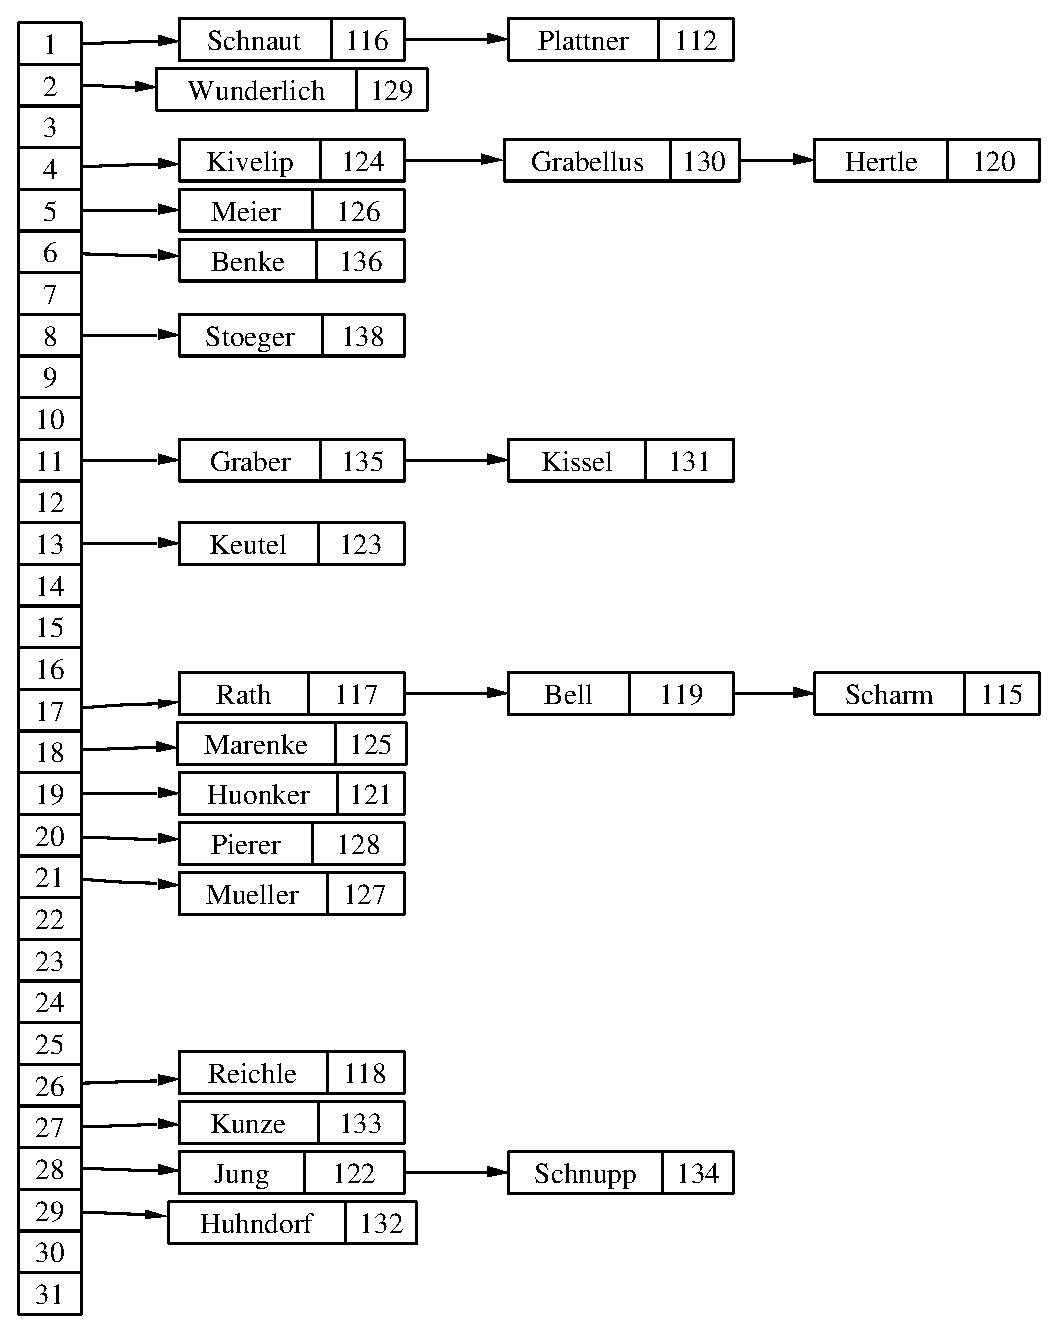
\epsfig{file=Abbildungen/hash-table,scale=0.6}} 
  \caption{A hash table.}
  \label{fig:hash-example}
\end{figure}

\noindent
Unfortunately, this naive implementation has several problems: 
\begin{enumerate}
\item The array needed to store the telephone dictionary has a size of 
      \\[0.2cm]
      \hspace*{1.3cm}
      $\ds 1 + \sum\limits_{i=0}^7 26 \cdot 27^i = 1 + 26 \cdot \frac{27^{7+1} - 1}{27 - 1} = 27^8 = 282,429,536,481$ 
      \\[0.2cm]
      entries.  If every entry needs 8 bytes, we would need more than two terabyte to store this array.
\item If two names happen to differ only after their eighth character, then we would not be able to
      store both of these names as we would not be able to distinguish between them.
\end{enumerate}
These problems can be solved as follows:
\begin{enumerate}
\item We have to change the function  $\texttt{code}$ so that the result of this function is always
      less than or equal to some given number $\texttt{size}$.  Here, the number $\texttt{size}$ specifies
      the number of entries of the array that we intend to use.  This number will be in the same
      order of magnitude as the number of key-value pairs that we want to store in our dictionary.

      There is a simple way to adapt the function  $\texttt{code}$ so that its result is never bigger
      than a given number $\texttt{size}$: If we define the function $\texttt{code}$ as
      \\[0.2cm]
      \hspace*{1.3cm} 
      $\ds\texttt{code}(c_0c_1\cdots c_n) = \left(\sum\limits_{i=0}^n \texttt{ord}(c_i) \cdot
        27^i\right) \;\texttt{\%}\; \texttt{size}$,
      \\[0.2cm]
      then we will always have $\texttt{code}(c_0c_1\cdots c_n) < \texttt{size}$.  
\item Rather than storing the values associated with the keys in an array, the values are now stored
      in \blue{lists} that contain key-value pairs.  The array itself only stores pointers to these
       lists. 
      
      The reason we have to use lists is the fact that different keys may be mapped to the
      same index.  Hence, we can no longer store the values directly in the array.  Instead,
      the values of all keys that map to the same index are stored in a
      list of key-value pairs.  These  lists are then stored in the array.  As long as
      these lists contain only a few entries, the look-up of a key is still fast: Given a key $k$,
      we first compute 
      \\[0.2cm]
      \hspace*{1.3cm}
      $\texttt{idx} = \texttt{code}(k)$.
      \\[0.2cm]
      Then, $\texttt{array}[\texttt{idx}]$ returns a list containing a pair of the form $\langle k, v \rangle$.
      In order to find the value associated with the key $k$ we have to search this list for the key
      $k$.
\end{enumerate}

\subsection{Computing the Hash Function Efficiently}
In this section we discuss how to compute the function 
\\[0.2cm]
\hspace*{1.3cm}
$\texttt{hash\_code}:\Sigma^* \rightarrow \mathbb{N}$
\\[0.2cm]
that takes a string $s$ and returns a natural number less than some predefined size $n$.
Given an \textsc{Ascii} string $s = c_0 c_1 c_2 \cdots c_{k-1}$ of length $k$ this function is defined as
\begin{equation}
  \texttt{hash\_code}(c_0c_1\cdots c_{k-1}, n) = \left(\sum\limits_{i=0}^{k-1} \texttt{ord}(c_i) \cdot 128^i\right) \mmod n.
  \label{eq:hash1}
\end{equation}
However, a naive implementation of equation (\ref{eq:hash1}) is inefficient because the computation of $128^i$
produces very big numbers.  In the programming language \texttt{C}, computing $128^i$ causes an overflow for a
string that has more than five characters.  In \textsl{Python}, integers are only bounded by the size of the
available memory and therefore overflow ist not a problem.  However, a computation
involving numbers with hundreds of places is considerably slower than a computation that uses numbers that fit
into a single memory word. Hence we should try to reorganize the computation that takes place in equation
(\ref{eq:hash1}).  This should be possible as the final result of $\texttt{hash\_code}(c_0c_1\cdots c_{k-1}, n)$
is bounded by $n$.  In order to be able to reorganize this computation we need to discuss
\href{https://en.wikipedia.org/wiki/Euclidean_division}{Euclidean division}.

\begin{Theorem}[Euclidean Division]
  Given two natural numbers $a, n \in \mathbb{N}$ such that $n > 0$, there exist \textbf{unique} natural numbers 
  $q$ and $r$ such that:
  \begin{enumerate}[(a)]
  \item $a = q \cdot n + r$ \quad and
  \item $0 \leq r < n$.
  \end{enumerate}
  The number $q$ is called the \blue{quotient} of $a$ divided $n$ and denoted as $a \;\texttt{//}\; n$, while
  $r$ is called the \blue{remainder} of $a$ divided by $n$ and denoted as $a \mmod n$.  \eox
\end{Theorem}

The existential claim of this theorem can be established by providing a program that computes $a \;\texttt{//}\; n$ and $a \mmod n$.  
A trivial way to do compute $a \mdiv n$ is to successively subtract
$n$ from $a$ as long as the result of the subtraction is non-negative.  Then $a \;\texttt{//}\; n$ is the number of times $n$ can be
subtracted from $a$.  Figure \ref{fig:Division-Naive.ipynb} shows an implementation of this idea.

\begin{figure}[!ht]
\centering
\begin{minted}[ frame         = lines, 
                 framesep      = 0.3cm, 
                 firstnumber   = 1,
                 bgcolor       = sepia,
                 numbers       = left,
                 numbersep     = -0.2cm,
                 xleftmargin   = 0.8cm,
                 xrightmargin  = 0.8cm,
               ]{python3}
    def divide(a, n):
        q = 0
        while a >= n:
            a -= n
            q += 1
        return q, a
\end{minted}
\vspace*{-0.3cm}
\caption{A naive implementation of Euclidean division.}
\label{fig:Division-Naive.ipynb}
\end{figure}
\exercise
Prove the uniqueness of the quotient and the remainder in the theorem on Euclidean division.
In order to do this, assume that
\begin{enumerate}
\item $a = q_1 \cdot n + r_1 = q_2 \cdot n + r_2$ and
\item $0 \leq r_1 < n$ and $0 \leq r_2 < n$
\end{enumerate}
holds and prove that this implies both $q_1 = q_2$ as well as $r_1 = r_2$.  \eox

When computing a sum $(a + b) \mmod n$ and $b$ is a big number, the following theorem can be used to simplify
the computation.

\begin{Theorem}[Modulo Arithmetic: Addition]
  If $a, b \in \mathbb{N}$ and $n \in \mathbb{N}$ with $n > 0$, then we have
  \\[0.2cm]
  \hspace*{1.3cm}
  $\ds (a + b) \mmod n = (a + b \mmod n) \mmod n$.
\end{Theorem}

\proof
If we define $q_1 := (a + b) \mdiv n$, then according to the division theorem we have 
\\[0.2cm]
\hspace*{1.3cm}
$a + b = q_1 \cdot n + (a + b) \mmod n$. 
\\[0.2cm]
Similarly, if $q_2 := b \mdiv n$ we have
\\[0.2cm]
\hspace*{1.3cm}
$b = q_2 \cdot n + b \mmod n$,
\\[0.2cm]
which implies that $b \mmod n = b - q_2 \cdot n$.
Therefore we have
\\[0.2cm]
\hspace*{1.3cm}
$
\begin{array}[t]{lcl}
  a + b \mmod n & = & a + b - q_2 \cdot n \\
                & = & q_1 \cdot n + (a + b) \mmod n - q_2 \cdot n \\
                & = & (q_1 - q_2) \cdot n + (a + b) \mmod n
\end{array}
$
\\[0.2cm]
Hence we have shown that
\\[0.2cm]
\hspace*{1.3cm}
$a + b \mmod n = (q_1 - q_2) \cdot n + (a + b) \mmod n$.
\\[0.2cm]
The right hand side of this equation has the same form as the first condition in the Euclidean division theorem.
As we also have $0 \leq (a + b) \mmod n < n$, the uniqueness of Euclidean division implies that
\\[0.2cm]
\hspace*{1.3cm}
$(a + b \mmod n) \mmod n = (a + b) \mmod n$
\\[0.2cm]
holds.  \qed

\begin{Theorem}[Modulo Arithmetic: Multiplication] \lb
  If $a, b \in \mathbb{N}$ and $n \in \mathbb{N}$ with $n > 0$, then we have
  \\[0.2cm]
  \hspace*{1.3cm}
  $\ds (a \cdot b) \mmod n = \bigl(a \cdot (b \mmod n)\bigr) \mmod n$.
\end{Theorem}

\exercise
Prove the last theorem. \eox

Next, we assume to have been given a finite sequence of numbers $a_0$, $a_1$, $a_2$, $\cdots$, $a_m$  and we want to compute the expression
\\[0.2cm]
\hspace*{1.3cm}
$\ds p(x) := \biggl(\sum\limits_{i=0}^m a_i \cdot x^i\biggr) \mmod n$.
\\[0.2cm]
\href{https://en.wikipedia.org/wiki/Horner%27s_method}{Horner's method}
for modular arithmetic is an efficient way to do this.  This method is introduced in the following theorem.

\begin{Theorem}[Horner's Method for Modular Arithmetic]
   Assume that $a_0$, $a_1$, $a_2$, $\cdots$, $a_m$ is a finite sequence of natural numbers, $x \in \mathbb{N}$,
   and $n\in \mathbb{N}$ such that $n > 0$.
   We define the sequence $s_k$ for $k=0,1,\cdots,m$ inductively as follows:
   \begin{description}
   \item[B.C.:] $k = 0$
             \\[0.2cm]
             \hspace*{1.3cm}
             $s_0 := a_m \mmod n$.
   \item[I.S.:] $k \mapsto k + 1$
             \\[0.2cm]
             \hspace*{1.3cm}
             $s_{k+1}:= (s_k \cdot x + a_{m - (k + 1)}) \mmod n$.
   \end{description}
   Then we have 
   \\[0.2cm]
   \hspace*{1.3cm}
   $\ds s_k = \biggl(\sum\limits_{i=0}^k a_{m - i} \cdot x^{k - i}\biggr) \mmod n$.
\end{Theorem}

\proof
As the numbers $s_m$ are defined by induction, the proof of this theorem is by
induction on $m$.
\begin{enumerate}
\item[B.C.:] $k = 0$
             \\[0.2cm]
             \hspace*{1.3cm}
           $\ds\biggl(\sum\limits_{i=0}^0 a_{m-i} \cdot x^{0-i}\biggr) \mmod n = \bigl(a_{m-0} \cdot x^0
          \bigr)\mmod n = a_m \mmod n = s_0$. $\surd$
\item[I.S.:] $k \mapsto k + 1$
             \\[0.2cm]
             \hspace*{1.3cm}
             $
             \begin{array}{lcll}
               s_{k+1} & = & (s_k \cdot x + a_{m - (k+1)} ) \mmod n \\[0.2cm]
                      & \stackrel{IV}{=} & \ds\Biggl(\biggl(\Bigl(\sum\limits_{i=0}^k a_{m-i} \cdot x^{k-i} \Bigr) \mmod n\biggr) \cdot x + a_{m - (k+1)}\Biggr) \mmod n
                                         \\[0.5cm]
                      & = & \ds\Biggl(\biggl(\sum\limits_{i=0}^k a_{m-i} \cdot x^{k-i} \Bigr) \cdot x + a_{m - (k+1)}\Biggr) \mmod n
                            \\[0.5cm]
                      & = & \ds\Biggl(\sum\limits_{i=0}^k a_{m-i} \cdot x^{k+1-i}  + a_{m - (k+1)} \cdot x^{k+1-(k+1)}\Biggr) \mmod n
                            \\[0.5cm]
                      & = & \ds\Biggl(\sum\limits_{i=0}^{k+1} a_{m-i} \cdot x^{k+1-i}  \Biggr) \mmod n \quad \surd & \Box
             \end{array}
             $
\end{enumerate}
Setting $k := m$ in Horner's method we arrive at the following formula:
\\[0.2cm]
\hspace*{1.3cm}
$\ds s_m = \biggl(\sum\limits_{i=0}^m a_{m - i} \cdot x^{m - i}\biggr) \mmod n = \biggl(\sum\limits_{i=0}^m a_{i} \cdot x^{i}\biggr) \mmod n = p(x)$.
\\[0.2cm]
This formula is used to implement the function \texttt{hash\_code} efficiently.
Figure \ref{fig:hash_code.py} shows an implementation of this formula.  We have set 
$x$ to $128$ here since $128$ is the size of the \textsc{Ascii} alphabet.

\subsection{Implementing Hash Tables}
In order to implement a has table we first need to implement three auxiliary classes:
\begin{enumerate}
\item We implement the class \texttt{ListNode} that represents the node of a linked list.
\item We implement the class \texttt{ListMap} that turns a linked list into a \blue{Map}.
\item We implement  the class \texttt{MapIterator} that is needed to iterate over a linked list.
\end{enumerate}

\subsubsection{The class \texttt{ListNode}}
We start by defining the class \texttt{ListNode}.
The implementation is shown in Figure \ref{fig:ListNode.ipynb} on page \pageref{fig:ListNode.ipynb}.
An object of class \texttt{ListNode} stores a key, a value, and a pointer to the next node.
\begin{enumerate}[(a)]
\item \texttt{mKey}     stores the \emph{key},
\item \texttt{mValue}   stores the \emph{value} associated with this key, and
\item \texttt{mNextPtr} stores a reference to the next node.  If there is no next node, then 
      \texttt{mNextPtr} is \texttt{None}.
\end{enumerate}

\begin{figure}[!ht]
\centering
\begin{minted}[ frame         = lines, 
                framesep      = 0.3cm, 
                firstnumber   = 1,
                bgcolor       = sepia,
                numbers       = left,
                numbersep     = 0.2cm,
                xleftmargin   = 0.8cm,
                xrightmargin  = 0.8cm,
              ]{python3}
    class ListNode:
        def __init__(self, key, value):
            self.mKey     = key
            self.mValue   = value
            self.mNextPtr = None                
\end{minted}
\vspace*{-0.3cm}
\caption{The constructor of the class \texttt{ListNode}.}
\label{fig:ListNode.ipynb}
\end{figure}

Given a \texttt{key}, the method \texttt{find} shown in Figure \ref{fig:ListNode.ipynb:find} traverses the
given linked list that starts at the node \texttt{self} until it finds a node that stores the 
given \texttt{key}.  In this case, it returns the associated value.  Otherwise, \texttt{None} is returned.

\begin{figure}[!ht]
\centering
\begin{minted}[ frame         = lines, 
                framesep      = 0.3cm, 
                firstnumber   = 1,
                bgcolor       = sepia,
                numbers       = left,
                numbersep     = -0.2cm,
                xleftmargin   = 0.8cm,
                xrightmargin  = 0.8cm,
              ]{python3}
def find(self, key):
    while True:
        if self.mKey == key:
            return self.mValue
        if self.mNextPtr != None:
            self = self.mNextPtr
        else:
            return
\end{minted}
\vspace*{-0.3cm}
\caption{The method \texttt{find} of the class \texttt{ListNode}.}
\label{fig:ListNode.ipynb:find}
\end{figure}

Given the first node of a \blue{linked list} $L$, the function $L.\texttt{insert}(k, v)$ shown in Figure
\ref{fig:ListNode.ipynb:insert} on page \pageref{fig:ListNode.ipynb:insert} inserts the key-value pair $(k, v)$
into the list $L$.  If there is already a key value pair in $L$ that has the same key, then the old value is
overwritten.  It returns a boolean that is true if a new node has been allocated.  This information is needed
later in order to keep track of the number of nodes in a linked list.

\begin{figure}[!ht]
\centering
\begin{minted}[ frame         = lines, 
                framesep      = 0.3cm, 
                firstnumber   = 1,
                bgcolor       = sepia,
                numbers       = left,
                numbersep     = -0.2cm,
                xleftmargin   = 0.8cm,
                xrightmargin  = 0.8cm,
              ]{python3}
    def insert(self, key, value):
        while True:
            if self.mKey == key:
                self.mValue = value
                return False
            elif self.mNextPtr != None:
                self = self.mNextPtr
            else:
                self.mNextPtr = ListNode(key, value)
                return True
\end{minted}
\vspace*{-0.3cm}
\caption{The method \texttt{insert} of the class \texttt{ListNode}.}
\label{fig:ListNode.ipynb:insert}
\end{figure}

Given the first node of a \blue{linked list} $L$, the method $L.\texttt{delete}(k)$ shown in Figure
\ref{fig:ListNode.ipynb:delete} on page \pageref{fig:ListNode.ipynb:delete} removes the first
key-value pair of the form $(k, v)$ from the list $L$.  If there is no such pair, the list $L$ is left unchanged.
The expression  $L.\texttt{delete}(k)$ returns a pair:
\begin{enumerate}[(a)]
\item The first component of this pair is a pointer to the resulting list.  If the list becomes empty, the
      first component is \texttt{None}.  
\item The second component is a Boolean that is \texttt{True} if a node has been deleted.
\end{enumerate}
In the implementation, the variable \texttt{previous} is a pointer to the object of class \texttt{ListNode}
that points to the node \texttt{self}.  For the first node, this pointer is \texttt{None}, but when we step
from one node to the next, this pointer is updated.  When we find the \texttt{key} that is to be deleted, there are
essentially two cases:
\begin{enumerate}
\item The \texttt{key} to be deleted is contained in the first node of the linked list.  In this case, \texttt{previous}
      is still \texttt{None}.  Therefore, we return a pointer to the rest of the list and set the Boolean
      that is returned to \texttt{True}.
\item Otherwise, we have to connect the node preceding the given node with the node succeeding the given node.
      This is done by setting \texttt{previous.mNextPtr} to \texttt{ptr.mNextPtr}.
      In this case, we return the pair $(\mathtt{self}, \mathtt{True})$ since \texttt{self} still points to the
      beginning of the list.
\end{enumerate}
As long as we have not found the \texttt{key}, we keep following the pointer \texttt{ptr.mNextPtr} to iterate over the
elements of the linked list.  If we reach the end of the list without finding the \texttt{key}, the pair
$(\mathtt{self}, \mathtt{False})$ is returned.

\begin{figure}[!ht]
\centering
\begin{minted}[ frame         = lines, 
                framesep      = 0.3cm, 
                firstnumber   = 1,
                bgcolor       = sepia,
                numbers       = left,
                numbersep     = -0.2cm,
                xleftmargin   = 0.8cm,
                xrightmargin  = 0.8cm,
              ]{python3}
    def delete(self, key):
        previous = None
        ptr      = self
        while True:
            if ptr.mKey == key:
                if previous == None:
                    return ptr.mNextPtr, True
                else:
                    previous.mNextPtr = ptr.mNextPtr
                    return self, True
            elif ptr.mNextPtr != None:
                previous = ptr
                ptr      = ptr.mNextPtr
            else:
                break
        return self, False
\end{minted}
\vspace*{-0.3cm}
\caption{The method \texttt{delete} of the class \texttt{ListNode}.}
\label{fig:ListNode.ipynb:delete}
\end{figure}
\subsubsection{The class \texttt{ListMap}}
\begin{figure}[!ht]
\centering
\begin{minted}[ frame         = lines, 
                framesep      = 0.3cm, 
                firstnumber   = 1,
                bgcolor       = sepia,
                numbers       = left,
                numbersep     = -0.2cm,
                xleftmargin   = 0.8cm,
                xrightmargin  = 0.8cm,
              ]{python3}
    class ListMap:
        def __init__(self):
            self.mPtr = None
            
        def find(self, key):
            if self.mPtr != None:
                return self.mPtr.find(key)
            
        def insert(self, key, value):
            if self.mPtr != None:
                return self.mPtr.insert(key, value)
            else:
                self.mPtr = ListNode(key, value)
                return True
                
        def delete(self, key):
            if self.mPtr != None:
                newPtr, flag = self.mPtr.delete(key)
                self.mPtr    = newPtr
                return flag
            return False
                
        def __iter__(self):
            return MapIterator(self.mPtr)
\end{minted}
\vspace*{-0.3cm}
\caption{The class \texttt{ListMap}.}
\label{fig:ListMap.ipynb}
\end{figure}

Now we are ready to present the class \texttt{ListMap} that implements the abstract data type \blue{Map} using a
linked list.  Figure \ref{fig:ListMap.ipynb} on page \pageref{fig:ListMap.ipynb} shows the implementation.
\begin{enumerate}[(a)]
\item The class maintains the  member variable \texttt{mPtr}, which is a pointer to the first node of a linked
      list.  As long as the list is empty, this pointer is \texttt{None}.

      Basically, the class \texttt{ListMap} is a wrapper for the class \texttt{ListNode} that is needed to deal
      with empty lists.
\item The method \texttt{find} is a wrapper of the method \texttt{find} from the class \texttt{ListNode}.
      If \texttt{mPtr} is set, then the linked list at \texttt{mPtr} is searched for the given \texttt{key}.
      Otherwise, the list is empty and \texttt{None} is returned.
\item The method \texttt{insert} is a wrapper of the method \texttt{insert} from the class \texttt{ListNode}.
      If \texttt{mPtr} is set, then the given \texttt{key}-\texttt{value} pair is inserted into the
      linked list specified by \texttt{mPtr}.
      Otherwise, a new \texttt{ListNode} is created that stores the given  \texttt{key}-\texttt{value}.
      In this case, the method has to return \texttt{True} since a new key has been inserted.
\item Similarly, the method \texttt{delete} is a wrapper of the method \texttt{delete} from the class
      \texttt{ListNode}.  If the given list is not empty, i.e. \texttt{mPtr} is not \texttt{None},
      the implementation tries to delete the given \texttt{key} in the list pointed to by \texttt{self.mPtr}.
      Care has to be taken for the case that the \texttt{key} to be deleted is the first node of the
      list pointed to by \texttt{mPtr}.  In this case, the value of \texttt{mPtr} will change.
\item Furthermore, the class implements the function \texttt{\_\_iter\_\_} which returns a
      \texttt{MapIterator}.  Therefore, an object of class \texttt{ListMap} is \blue{iterable}: We can
      use a \texttt{for}-loop to iterate over the list that is stored.  
\end{enumerate}
\subsubsection{The class \texttt{MapIterator}}
Next, we discuss the class \texttt{MapIterator} which makes \texttt{ListMap} objects iterable.
This class is shown in Figure \ref{fig:MapIterator.ipynb} on page \pageref{fig:MapIterator.ipynb}.
This class maintains a pointer to the next list node that is to be returned by this iterator.
The constructor sets this pointer to the first node of the associated linked list.
The method \texttt{\_\_next\_\_} is responsible for retrieving a key-value pair and updating this pointer.
If the end of the list is reached, then this method raises a \texttt{StopIteration}, which signals that the
list has been exhausted.

\begin{figure}[!ht]
\centering
\begin{minted}[ frame         = lines, 
                framesep      = 0.3cm, 
                firstnumber   = 1,
                bgcolor       = sepia,
                numbers       = left,
                numbersep     = -0.2cm,
                xleftmargin   = 0.8cm,
                xrightmargin  = 0.8cm,
              ]{python3}
    class MapIterator:
        def __init__(self, ptr):
            self.mPtr = ptr
        
        def __next__(self):
            if self.mPtr == None:
                raise StopIteration
            key   = self.mPtr.mKey
            value = self.mPtr.mValue
            self.mPtr = self.mPtr.mNextPtr
            return key, value
\end{minted}
\vspace*{-0.3cm}
\caption{The class \texttt{MapIterator}.}
\label{fig:MapIterator.ipynb}
\end{figure}


\subsubsection{The class \texttt{HashMap}}
In order to implement a hash table we need a hash function.  Figure \ref{fig:hash_code.py} on page
\pageref{fig:hash_code.py} shows the function \texttt{hash\_code}.
Given a string $w$ and the size $n$ of the hash table, the function $\texttt{hash\_code}(w, n)$ calculates the
hash code of $w$.  For a string  
$w = c_0c_1\cdots c_{m-1}$ of length $m$, this function is defined as follows:
$$ \texttt{hash\_code}(w, n) = \left(\sum\limits_{i=0}^{m-1} \texttt{ord}(c_i) \cdot 128^i\right) \;\texttt{\symbol{37}}\; n  $$
In order to prevent overflows when computing the numbers $128^i$ we can define the partial sum $s_k$ for
$k=0,1,\cdots,m-1$ by induction:
\begin{enumerate}[(a)]
\item $s_{0} = \texttt{ord}(c_{m-1}) \;\texttt{\symbol{37}}\; n$,
\item $s_{k+1} = \bigl(s_k \cdot 128 + \texttt{ord}(c_{k}) \bigr) \;\texttt{\symbol{37}}\; n$.
\end{enumerate}
Then we have
\\[0.2cm]
\hspace*{1.3cm}
$s_{m-1} = \left(\sum\limits_{i=0}^{m-1} \texttt{ord}(c_i) \cdot 128^i\right) \;\texttt{\symbol{37}}\; n$.

\begin{figure}[!ht]
\centering
\begin{minted}[ frame         = lines, 
                framesep      = 0.3cm, 
                firstnumber   = 1,
                bgcolor       = sepia,
                numbers       = left,
                numbersep     = -0.2cm,
                xleftmargin   = 0.8cm,
                xrightmargin  = 0.8cm,
              ]{python3}
    def hash_code(w, n):
        m = len(w)
        s = 0
        for k in range(m-1, -1, -1):
            s = (s * 128 + ord(w[k])) % n
        return s
\end{minted}
\vspace*{-0.3cm}
\caption{The function \texttt{hash\_code} to compute a hash code for a string.}
\label{fig:hash_code.py}
\end{figure}
\pagebreak

\noindent
Figure \ref{fig:HashMap.ipynb} on page \pageref{fig:HashMap.ipynb} shows the class \texttt{HashMap}

\begin{figure}[!ht]
  \centering
\begin{minted}[ frame         = lines, 
                framesep      = 0.3cm, 
                bgcolor = sepia,
                numbers       = left,
                numbersep     = -0.2cm,
                xleftmargin   = 0.0cm,
                xrightmargin  = 0.0cm
              ]{python3}
    class HashTable:
        def __init__(self, n, code=hash_code):
            self.mSize    = n
            self.mEntries = 0                                        
            self.mArray   = [ ListMap() for i in range(self.mSize) ] 
            self.mAlpha   = 2                                        
            self.mCode    = code

    HashTable.Primes = [ 3, 7, 13, 31, 61, 127, 251, 509, 1021, 2039, 4093, 
                         8191, 16381, 32749, 65521, 131071, 262139, 524287, 
                         1048573, 2097143, 4194301, 8388593, 16777213, 
                         33554393, 67108859, 134217689, 268435399, 
                         536870909, 1073741789, 2147483647 
                       ]        
\end{minted}
\vspace*{-0.3cm}
  \caption{Definition of the class $\texttt{HashTable}$.}
  \label{fig:HashMap.ipynb}
\end{figure}

\begin{enumerate}
\item The constructor \texttt{\_\_init\_\_} is called with two arguments.
      \begin{enumerate}[(a)]
      \item This argument $n$ is the initial size of the array storing the \texttt{ListMaps} of key-value
            pairs.  The constructor constructs an empty hash table of size $n$.
      \item \texttt{code} is a function that takes an object and returns the hash code of this object.
            The default is to use the function \texttt{hash\_code} defined above.
      \end{enumerate}
\item $\texttt{mSize}$ is the actual size of the array that stores the different key-value lists.
      Although this variable is initialized as $n$, it can be increased later if more space is needed.  This happens 
      if the hash table becomes \blue{overcrowded}.
\item $\texttt{mEntries}$ is the number of key-value pairs that are stored in this hash map.
      Since, initially, this map is empty, $\texttt{mEntries}$ is  initialized as $0$.
\item $\texttt{mArray}$ is the array containing the list of key value pairs.
      As the hash map is initially empty, all entries of $\texttt{mArray}$ are initialized as empty \texttt{ListMap}s.
\item $\texttt{mAlpha}$ is the \blue{load factor} of our hash table.  If at any point in time we have that
      \\[0.2cm]
      \hspace*{1.3cm}
      $\texttt{mEntries} > \texttt{mAlpha} \cdot \texttt{mSize}$,
      \\[0.2cm]
      then we consider our hash table to be \blue{overcrowded}.  In that case, we increase the size
      of the array $\texttt{mArray}$.  To determine the best value for $\texttt{mAlpha}$, we have to
      make a tradeoff:  If $\texttt{mAlpha}$ is too big, many entries in the array $\texttt{mArray}$
      will be empty and thus we will waste space.  On the other hand, if $\texttt{mAlpha}$ is too
      small, the key-value lists will become very long and hence it will take too much time to
      search for a given key in one of these lists.
\item Our implementation maintains the static variable $\texttt{Primes}$.  This is a list of prime numbers.
      Roughly, these prime numbers double in size.   
      The reason is that the performance of a hash table is best if the size of $\texttt{mArray}$ is a
      prime number.  When the hash table gets overcrowded, the idea is to, more or less, double
      the size of $\texttt{mArray}$.  To achieve this, the variable $\texttt{sPrimes}$ is needed.
\end{enumerate}
Next, we discuss the implementation of the  methods of the class \texttt{HashTable}.

\begin{figure}[!ht]
\centering
\begin{minted}[ frame         = lines, 
                  framesep      = 0.3cm, 
                  firstnumber   = 1,
                  bgcolor = sepia,
                  numbers       = left,
                  numbersep     = -0.2cm,
                  xleftmargin   = 0.8cm,
                  xrightmargin  = 0.8cm,
                ]{python3}
    def find(self, key):
        index = self.mCode(key, self.mSize)
        aList = self.mArray[index];
        for k, v in aList:
            if k == key:
                return v
\end{minted}
\vspace*{-0.3cm}
\caption{Implementation of $\texttt{find}$.}
\label{fig:HashMap.ipynb-find}
\end{figure}

Figure \ref{fig:HashMap.ipynb-find} shows the implementation of the method $\texttt{find}$.
\begin{enumerate}
\item First, we compute the index of the \texttt{ListMap} that is used to store the given
      $\texttt{key}$.
\item Next, we retrieve this \texttt{ListMap} from the array $\texttt{mArray}$.
\item Finally, we look up the information stored under the given $\texttt{key}$ in this key-value list.
      Since the class \texttt{ListMap} is iterable we can use a \texttt{for}-loop to loop over the key-value
      pairs and return the value associated with the given \texttt{key}.
\end{enumerate}

\begin{figure}[!ht]
\centering
\begin{minted}[ frame         = lines, 
                  framesep      = 0.3cm, 
                  firstnumber   = 1,
                  bgcolor = sepia,
                  numbers       = left,
                  numbersep     = -0.2cm,
                  xleftmargin   = 0.8cm,
                  xrightmargin  = 0.8cm,
                ]{python3}
    def insert(self, key, value):
        if self.mEntries >= self.mSize * self.mAlpha:
            self._rehash()
        index = self.mCode(key, self.mSize)
        aList = self.mArray[index]
        self.mEntries += aList.insert(key, value)
\end{minted}
\vspace*{-0.3cm}
\caption{Implementation of the method $\texttt{insert}$.}
\label{fig:hashTable.ipython-insert}
\end{figure}

Figure \ref{fig:hashTable.ipython-insert} shows the implementation of the method $\texttt{insert}$.
The implementation works as follows.
\begin{enumerate}
\item First, we check whether our hash table is already overcrowded.
      In this case, we \blue{rehash}, which means we roughly double the size of $\texttt{mArray}$.
      How the method $\texttt{rehash}$ works in detail is explained later.
\item Next, we compute the index of the \texttt{ListMap} that has to store
      $\texttt{mKey}$, retrieve the associated \texttt{ListMap}, and finally insert the \texttt{key} and the
      \texttt{value} into this \texttt{ListMap}.
      When doing this we take care to maintain the correct number of entries.
\end{enumerate}


\begin{figure}[!ht]
\centering
\begin{minted}[ frame         = lines, 
                framesep      = 0.3cm, 
                firstnumber   = 1,
                bgcolor = sepia,
                numbers       = left,
                numbersep     = -0.2cm,
                xleftmargin   = 0.0cm,
                xrightmargin  = 0.0cm,
              ]{python3}
    def _rehash(self):
        for p in HashTable.Primes:
            if p * self.mAlpha > self.mEntries:
                prime = p
                break
        biggerTable = HashTable(prime, self.mCode)
        for aList in self.mArray:
            for k, v in aList:
                biggerTable.insert(k, v)
        self.mSize  = prime
        self.mArray = biggerTable.mArray
\end{minted}
\vspace*{-0.3cm}
\caption{Implementation of the method $\texttt{rehash}$.}
\label{fig:hashTable.ipython-rehash}
\end{figure}


Figure \ref{fig:hashTable.ipython-rehash} shows the implementation of the method
$\texttt{rehash}()$.  This method is called if the hash table becomes overcrowded.  The idea is to
roughly double the size of $\texttt{mArray}$.  Theoretical considerations that are  beyond the scope
of this lecture show that it is beneficial if the size of $\texttt{mArray}$ is a prime number.
Hence, we look for the first prime number $\texttt{prime}$ such that $\texttt{prime}$ times the load
factor $\texttt{mAlpha}$ is bigger than the
number of entries.  This will assure that after rehashing the average number of entries in each key-value
list is less than the load factor $\texttt{mAlpha}$.  After we have determined $\texttt{prime}$, we
proceed as follows: 
\begin{enumerate}
\item We create a new empty hash table of size $\texttt{prime}$.
\item Next, we insert the key-value pairs from the given hash table in our newly created new hash table
      \texttt{biggerTable}.
\item Finally, the array stored in the new hash table is moved to the given hash table
      and the size is adjusted correspondingly.
\end{enumerate}

\begin{figure}[!ht]
\centering
\begin{minted}[ frame         = lines, 
                framesep      = 0.3cm, 
                firstnumber   = last,
                bgcolor = sepia,
                numbers       = left,
                numbersep     = -0.2cm,
                xleftmargin   = 0.8cm,
                xrightmargin  = 0.8cm,
              ]{python3}
    def delete(self, key):
        if 2 * self.mEntries <= self.mSize * self.mAlpha:
            self._rehash()
        index = self.mCode(key, self.mSize)
        aList = self.mArray[index]
        self.mEntries -= aList.delete(key)
\end{minted}
\vspace*{-0.3cm}
\caption{Implementation of the procedure $\texttt{delete}(\texttt{map}, \texttt{key})$.}
\label{fig:HashMap.ipynb-delete}
\end{figure}

Finally, we discuss the implementation of the method $\texttt{delete}$ that is shown in Figure
\ref{fig:HashMap.ipynb-delete}.  The implementation of this method is similar to the implementation
of the method $\texttt{insert}$.  When the number of elements drops below a threshold that is dependent on the
site of \texttt{mArray}, the table shrinks in order to not use too much memory.

In the worst case, the complexity of
the methods  $\texttt{find}$, $\texttt{insert}$, and $\texttt{delete}$ can grow \blue{linearly} with the number
of entries in the hash table.  This happens if the function 
$\texttt{hash\_code}(k)$ returns the same number for all keys $k$.  Although this case is
highly unlikely, it is not impossible.  If we have a good function to compute hash codes, then
most of the  lists will have roughly the same length.  The average length of a list is then
 \\[0.2cm]
\hspace*{1.3cm}
 $\alpha = \ds \frac{\texttt{mEntries}}{\texttt{mSize}}$. 
\\[0.2cm]
Here, the number $\alpha$ is the \blue{load factor} of the hash table.  In practice, in order to
achieve good performance, $\alpha$ should be less than 4.  The implementation of the programming
language \textsl{Java} provides the class  $\texttt{HashMap}$ that implements maps via hash tables.
The default load factor used in this class is only $\texttt{0.75}$.

\subsection{Further Reading}
In this section, we have discussed hash tables only briefly.  The reason is that, although hash tables are very
important in practice, a thorough treatment requires quite a lot of mathematics, see for example the
third volume of Donald Knuth's ``The Art of Computer Programming'' \cite{knuth:1998b}.  For this
reason, the design of a hash function is best left for experts.  In practice, hash tables are
quite a bit faster than \blue{AVL}-trees or \blue{red-black} trees.  However, this is only true if
the hash function that is used is able to spread the keys uniformly.  If this assumption is
violated, the use of a hash table can lead to serious performance 
bugs.  If, instead, a good
implementation of red-black-trees is used, the program might be slower in general but is certain to
be protected from the ugly surprises that can result from a poor hash function.  My advice for the reader
therefore is to use hashing only if you are sure that your hash function distributes the keys evenly.


\section{Applications}
Both \texttt{C++} and \textsl{Java} provide maps.  In \texttt{C++}, maps are part of the standard
template library, while \textsl{Java} offers the interface \texttt{Map} that is implemented both by
the class $\texttt{TreeMap}$ and the class $\texttt{HashMap}$. Furthermore, all modern script languages provide maps.
For example, in \textsl{Perl} \cite{Wall92}, maps are known as \blue{associative arrays}, in \textsl{Lua} 
\cite{ierusalimschy:2006,Ieru96a} maps are called \blue{tables}, and in \textsl{Python} 
\cite{vanRossum:95,lutz:09} maps are called \blue{dictionaries}.  

Later, when we discuss Dijkstra's algorithm for finding the shortest path in a graph we will see an
application of maps.

\section{Check Your Understanding}
If you are able to answer the questions below confidently, then you can assume that you have mastered the concepts
introduced in this chapter.
\begin{enumerate}
\item How are sets related to maps?
\item What is the definition of the abstract data type Map?
\item Describe a practical application of the \textsc{Adt} Map.
\item How is the set $\mathcal{B}$ of \emph{ordered binary trees} defined?
\item How are the functions $\mathtt{find}$, $\mathtt{insert}$, and $\mathtt{delete}$ defined for ordered
      binary trees?
\item What is the average complexity of the function $\mathtt{find}$ for an ordered binary tree?
      What is the worst case complexity?
\item How is the set $\mathcal{A}$ of \textsc{Avl} trees defined?
\item How did we define the function $\mathtt{restore}$ that is used to maintain the balancing condition
      in \textsc{Avl} trees?
\item What is the worst case complexity of \textsc{Avl} trees?
\item When can we use tries to implement a map? How are tries defined?
\item How are the functions $\mathtt{find}$, $\mathtt{insert}$, and $\mathtt{delete}$ defined for tries?
\item How are binary tries defined?
\item Define hash tables.
\item How is the load factor of a hash table defined?
      What happens if the load factor gets too big?
\item Describe a simple method to compute the hash value of a string.
\end{enumerate}

%%% Local Variables: 
%%% mode: latex
%%% TeX-master: "algorithms"
%%% End: 
